We implemented GSACO-O algorithm in Python using PyTorch, as it handles tensor operations efficiently and provides a multiprocessing library for
parallelization, thus significantly speeding up the ants' execution of the GS procedure in each GSACO-O iteration.%
\footnote{The source code is publicly available in our GitHub repository:
	\url{https://github.com/prosysscience/GSACO}}
The first challenge consists of determining suitable values for the input
parameters listed in Table~\ref{tab:parameters}, i.e.,
all parameters but the internally calculated pheromone level $\tau_e$ on edges~$e$.
We adhere to the parameters specified in Table~\ref{tab:p_value}, setting a time constraint~$l$ of $10$ minutes for objective makespan and $5$ minutes for objective operations. 
Setting different time limits for these two aspects allows the algorithm to tailor its computational efforts to the specific demands of each task. While makespan optimization seeks the best possible sequence over all operations (requiring extensive computation), optimizing operational efficiency focuses on making quicker adjustments that enhance day-to-day operations without the need for extensive computation. 
For the SMSP instances derived from the SMT2020 dataset, we consider up to $5$ operations per job for minimizing makespan and up to $15$ operations per job for optimizing operational throughput. These parameters are practical, given the stochastic nature of the problem which often necessitates frequent rescheduling. Additionally, we define a short planning horizon~$h$ to accommodate near-term scheduling requirements.
For the initial pheromone level~$\tau_y$,
we start from value~$1$, and take $0.00001$ as the minimum $\tau_z$
to avoid going down to $0$, considering that the GS procedure can only
select edges with non-zero entries in the pheromone matrix.
The values for the number~$k$ of ants, the evaporation rate~$\rho$,
and the pheromone contribution~$c$ are more sophisticated to pick.
That is, we tuned these parameters in a trial-and-error process that,
starting from a baseline, inspects deviations of the final makespan and convergence speed obtained with iterative modifications.
Certainly, an automated approach would be desirable to
perform this task efficiently for new instance sets.%
%
\begin{table}[t]
	\caption{GSACO input parameter values}\label{tab:p_value} \centering
	\begin{tabular}{|l|l|}
		\hline
		Parameter & Value \\ \hline
		$o$ & makespan/operations        \\
		$l$ & $10/5$        \\
		$n$ & $1$--$5$/$15$ \\
		$h$ & $1$--$6$ \\
		$k$ & $10$ \\
		$\tau_{y}$ & $1$ \\
		$\tau_{z}$ & $0.00001$ \\
		%		$\alpha$ & 1  \\
		%		$\beta$ & 1     \\
		$\rho$ & $0.7$ \\
		$c$ & $0.5$ \\
		\hline
	\end{tabular}
\end{table}

To evaluate large-scale SMSP instances,
we consider two semiconductor production scenarios of the SMT2020 dataset:
Low-Volume/High-Mix (LV/HM) and High-Volume/Low-Mix (HV/LM).
As indicated in Table~\ref{tab:Dataset},
both scenarios include more than $2000$ jobs and more than $1300$ machines,
modeling the production processes of modern semiconductor fabs.
The main difference is given by the number of products and associated production routes for jobs, where LV/HM considers $10$ production routes varying between
$200$--$600$ steps in total, while HV/LM comprises $2$ production routes with about
$300$ or $600$ steps, respectively.
Originally, the LV/HM and HV/LM scenarios have been designed to represent fab load at the
start of simulation runs, so that the jobs are at different steps of their
production routes.
We focus on scheduling for operations~$n$ from~$1$ up to~$5$,
to be performed per job.
Hence, the operations $O$ to schedule gradually increase from the
number $J$ of jobs, in case of the operations $n=1$,
% , given in Table~\ref{tab:Dataset},
to more than $10000$ operations % obtained
for the longest % planning 
horizon $n=5$.

\begin{table}[t]
	\caption{Number of jobs, machines, and operations for SMSP instances}\label{tab:Dataset} \centering
	\begin{tabular}{|l|c|c|c|}
		\hline
		Scenario & $J$    & $M$    & $O$              \\ \hline
		LV/HM    & $2156$ & $1313$ & up to $10747$    \\ 
		HV/LM    & $2256$ & $1443$ & up to $11218$    \\
		\hline
	\end{tabular}
\end{table}
%

\begin{table*}[t]
	\caption{SMSP results obtained with CP and GSACO \cite{Ali2024}}\label{tab:results} \centering
	\begin{tabular}{|l|l|l|l|l|l|l|l|l|l|l|l|}
		\hline
		&
		&
		\multicolumn{2}{c|}{$1$ min} &
		\multicolumn{2}{c|}{$3$ min} &
		\multicolumn{2}{c|}{$5$ min} &
		\multicolumn{2}{c|}{$7$ min} &
		\multicolumn{2}{c|}{$9$ min} \\ \cline{3-12} 
		$n$ & Scenario & CP & GSACO & CP & GSACO & CP & GSACO & CP & GSACO & CP & GSACO \\ \hline
		\multirow{2}{*}{$1$} & LV/HM & - & $3735$ & $18572$ & $3725$ & $3746$ & $3725$ & $3723$ & $3725$ & $3723$ & $3725$  \\
		& HV/LM & - & $1405$ & - & $1405$ & $2242$ & $1405$ & $1609$ & $1405$ & $1600$ & $1405$ \\
		\multirow{2}{*}{$2$} & LV/HM & - & $3773$ & - & $3751$ & - & $3750$ & - & $3739$ & $4398$ & $3739$ \\
		& HV/LM & - & $1653$ & - & $1644$ & - & $1611$ & - & $1611$ & - & $1611$   \\
		\multirow{2}{*}{$3$} & LV/HM & - & $3880$ & - & $3867$ & - & $3836$ & - & $3834$ & - & $3834$   \\
		& HV/LM & - & $1902$ & - & $1889$ & - & $1889$ & - & $1876$ & - & $1876$     \\
		\multirow{2}{*}{$4$} & LV/HM & - & $4578$ & - & $4540$ & - & $4540$ & - & $4540$ & - & $4540$     \\
		& HV/LM & - & $2207$ & - & $2113$ & - & $2113$ & - & $2093$ & - & $2093$  \\
		\multirow{2}{*}{$5$} & LV/HM & - & $4680$ & - & $4680$ & - & $4553$ & - & $4553$ & - & $4553$   \\	
		& HV/LM & - & $2667$ & - & $2566$ & - & $2566$ & - & $2518$ & - & $2518$ \\
		\hline  
	\end{tabular}
\end{table*}

While running with a time limit $l$ of $10$ minutes,
Table~\ref{tab:results} reports the makespans of current best schedules
found by the CP solver OR-Tools and our GSACO implementation
at $1$, $3$, $5$, $7$, and $9$ minutes of computing time.
Considering that the SMSP instances are large,
OR-Tools now takes $3$ minutes to come up with the first solution(s)
for the shortest planning horizon $n=1$ on the LV/HM scenario.
Within the same fraction of computing time, GSACO-O already converges to a
makespan of $3725$ and then proceeds with iterations that do not
yield further improvements.
That the best schedule found by GSACO is not optimal is witnessed by a
marginally better solution obtained by OR-Tools after $7$ minutes.
However, for the other SMSP instances, OR-Tools is unable to improve over
GSACO within $9$ minutes, and it cannot even provide feasible schedules
for planning horizons from $n=2$ on the HV/LM scenario or $n=3$ 
on LV/HM.
We performed our experiments on a TUXEDO Pulse 14 Gen1 machine
equipped with an 8-core AMD Ryzen 7 4800H processor at 2.9GHz and onboard
Radeon graphics card.

\begin{figure*}[t]
	\centering
	\begin{subfigure}[b]{0.45\linewidth}
		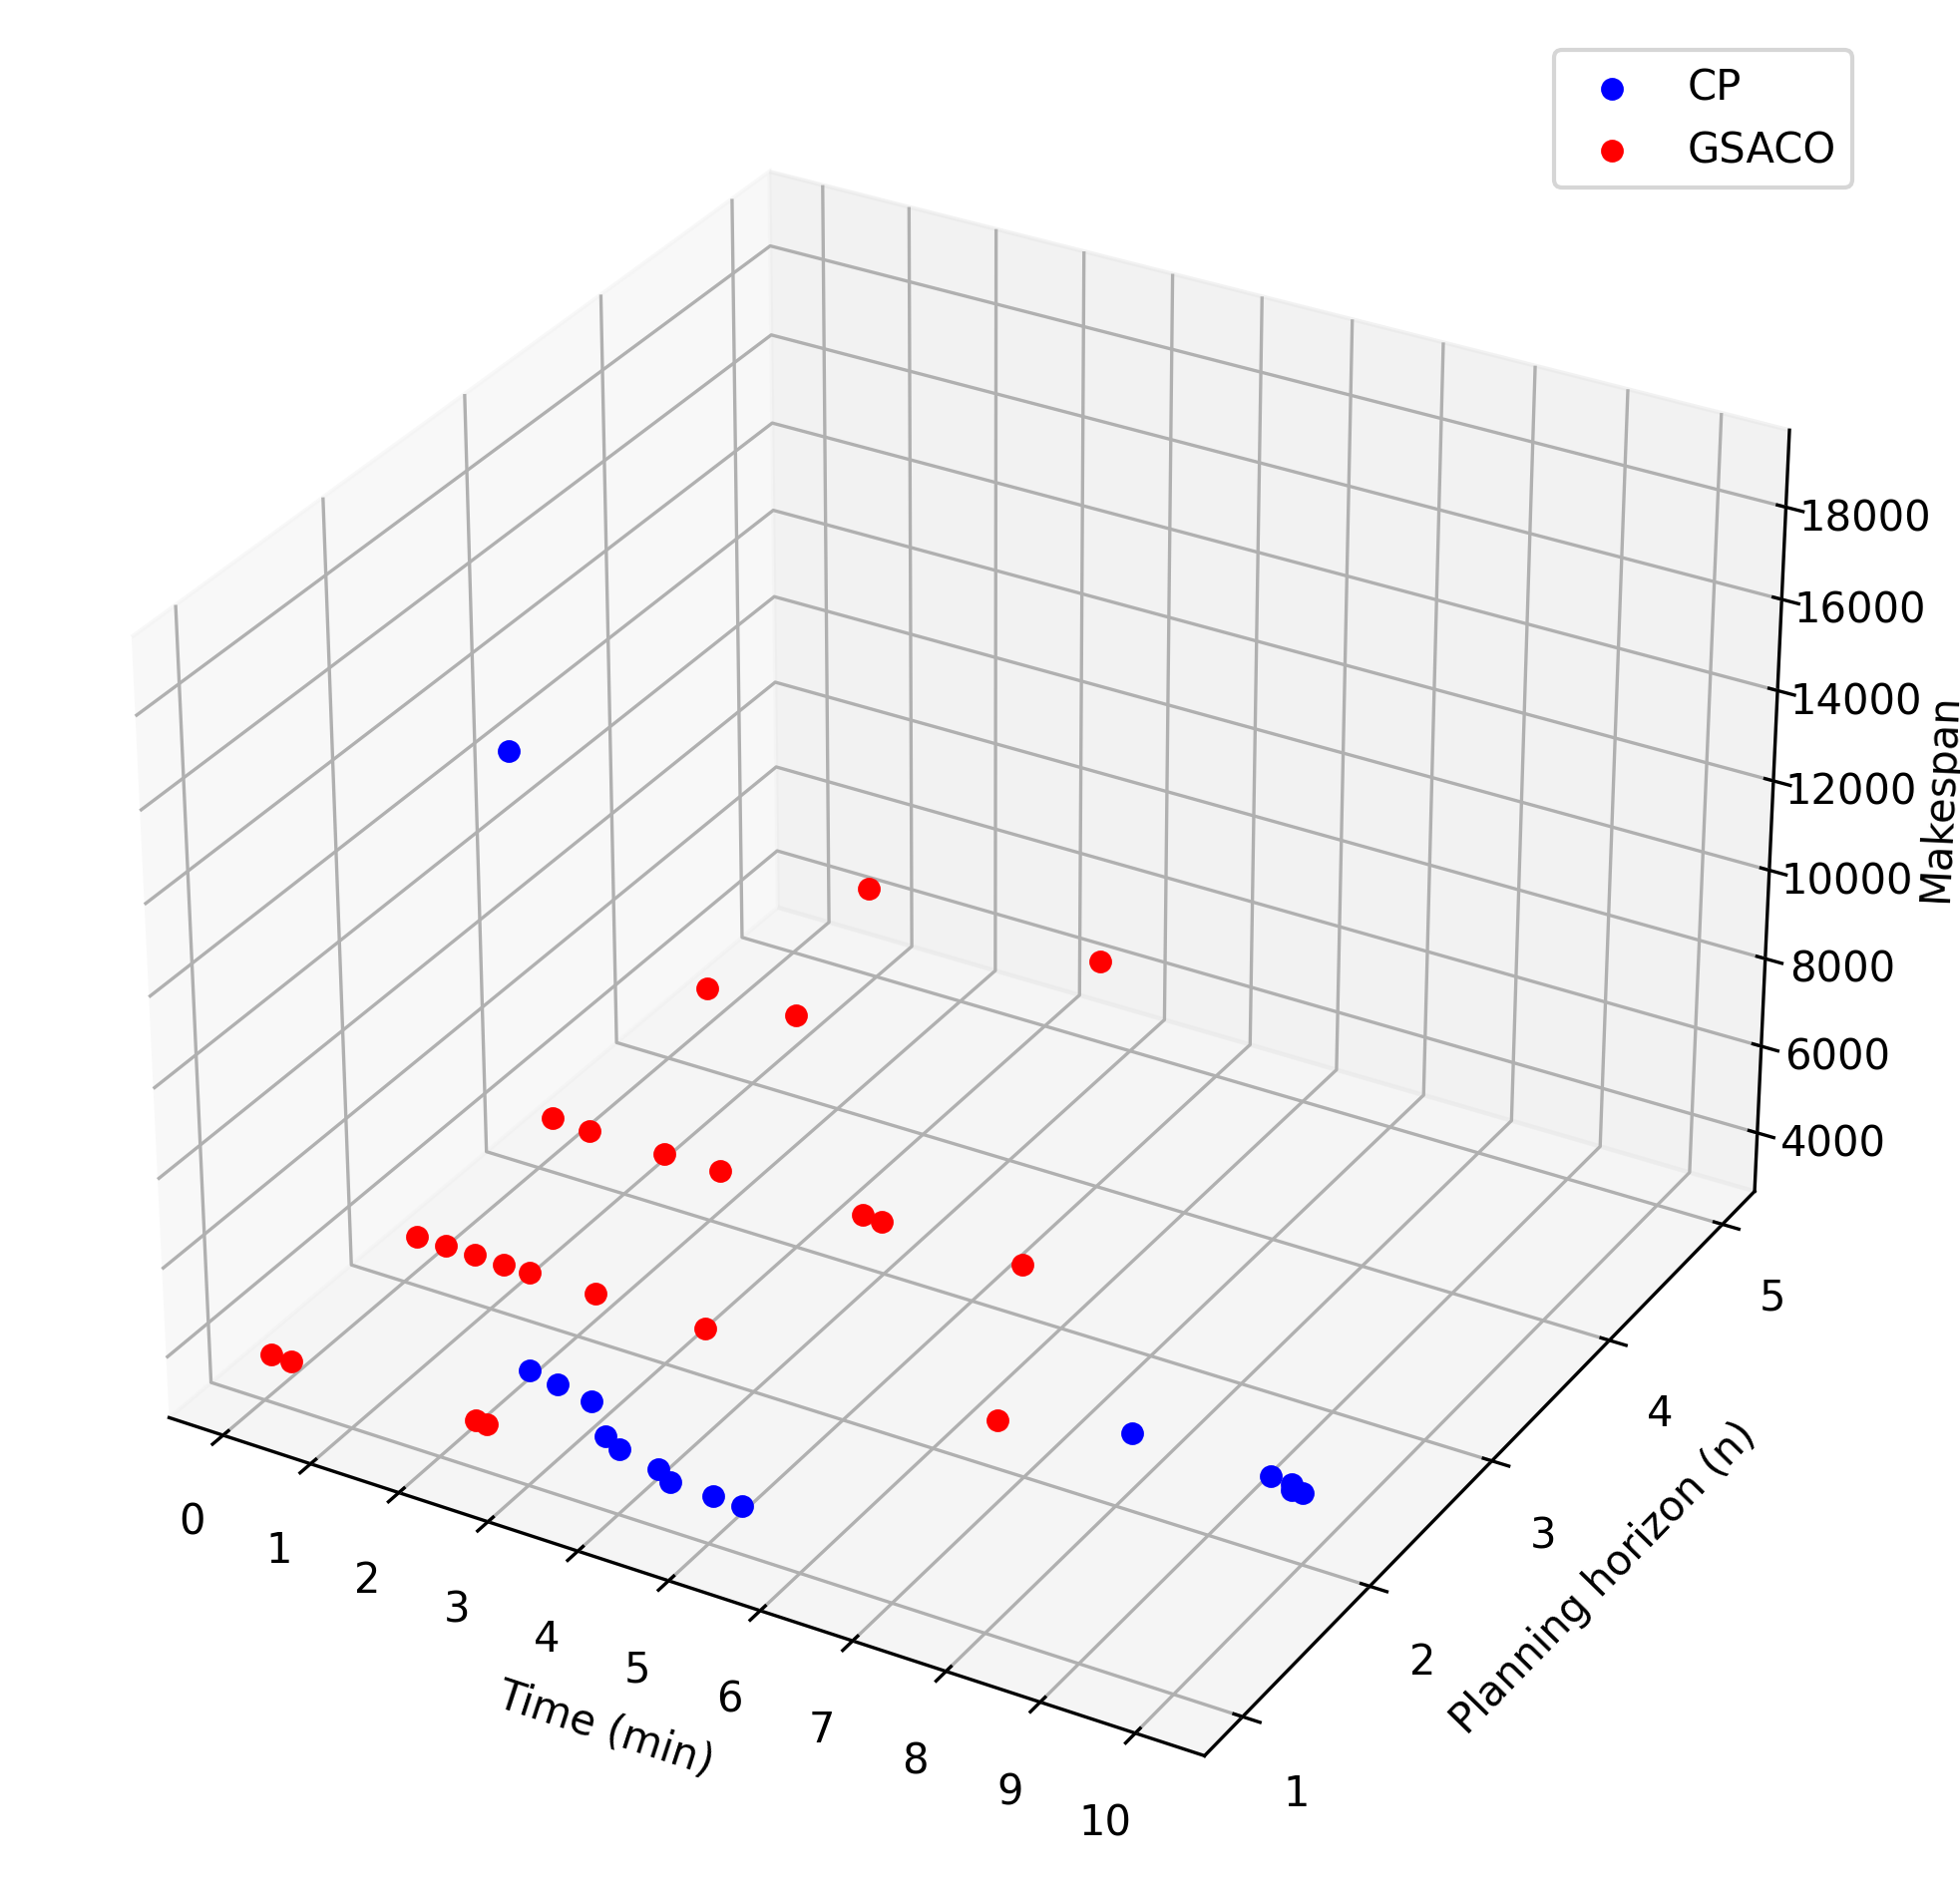
\includegraphics[width=\textwidth]{LVHM.png}
		\caption{LV/HM scenario}
		\label{subfig:l}
	\end{subfigure}
	\hfill
	\begin{subfigure}[b]{0.45\linewidth}
		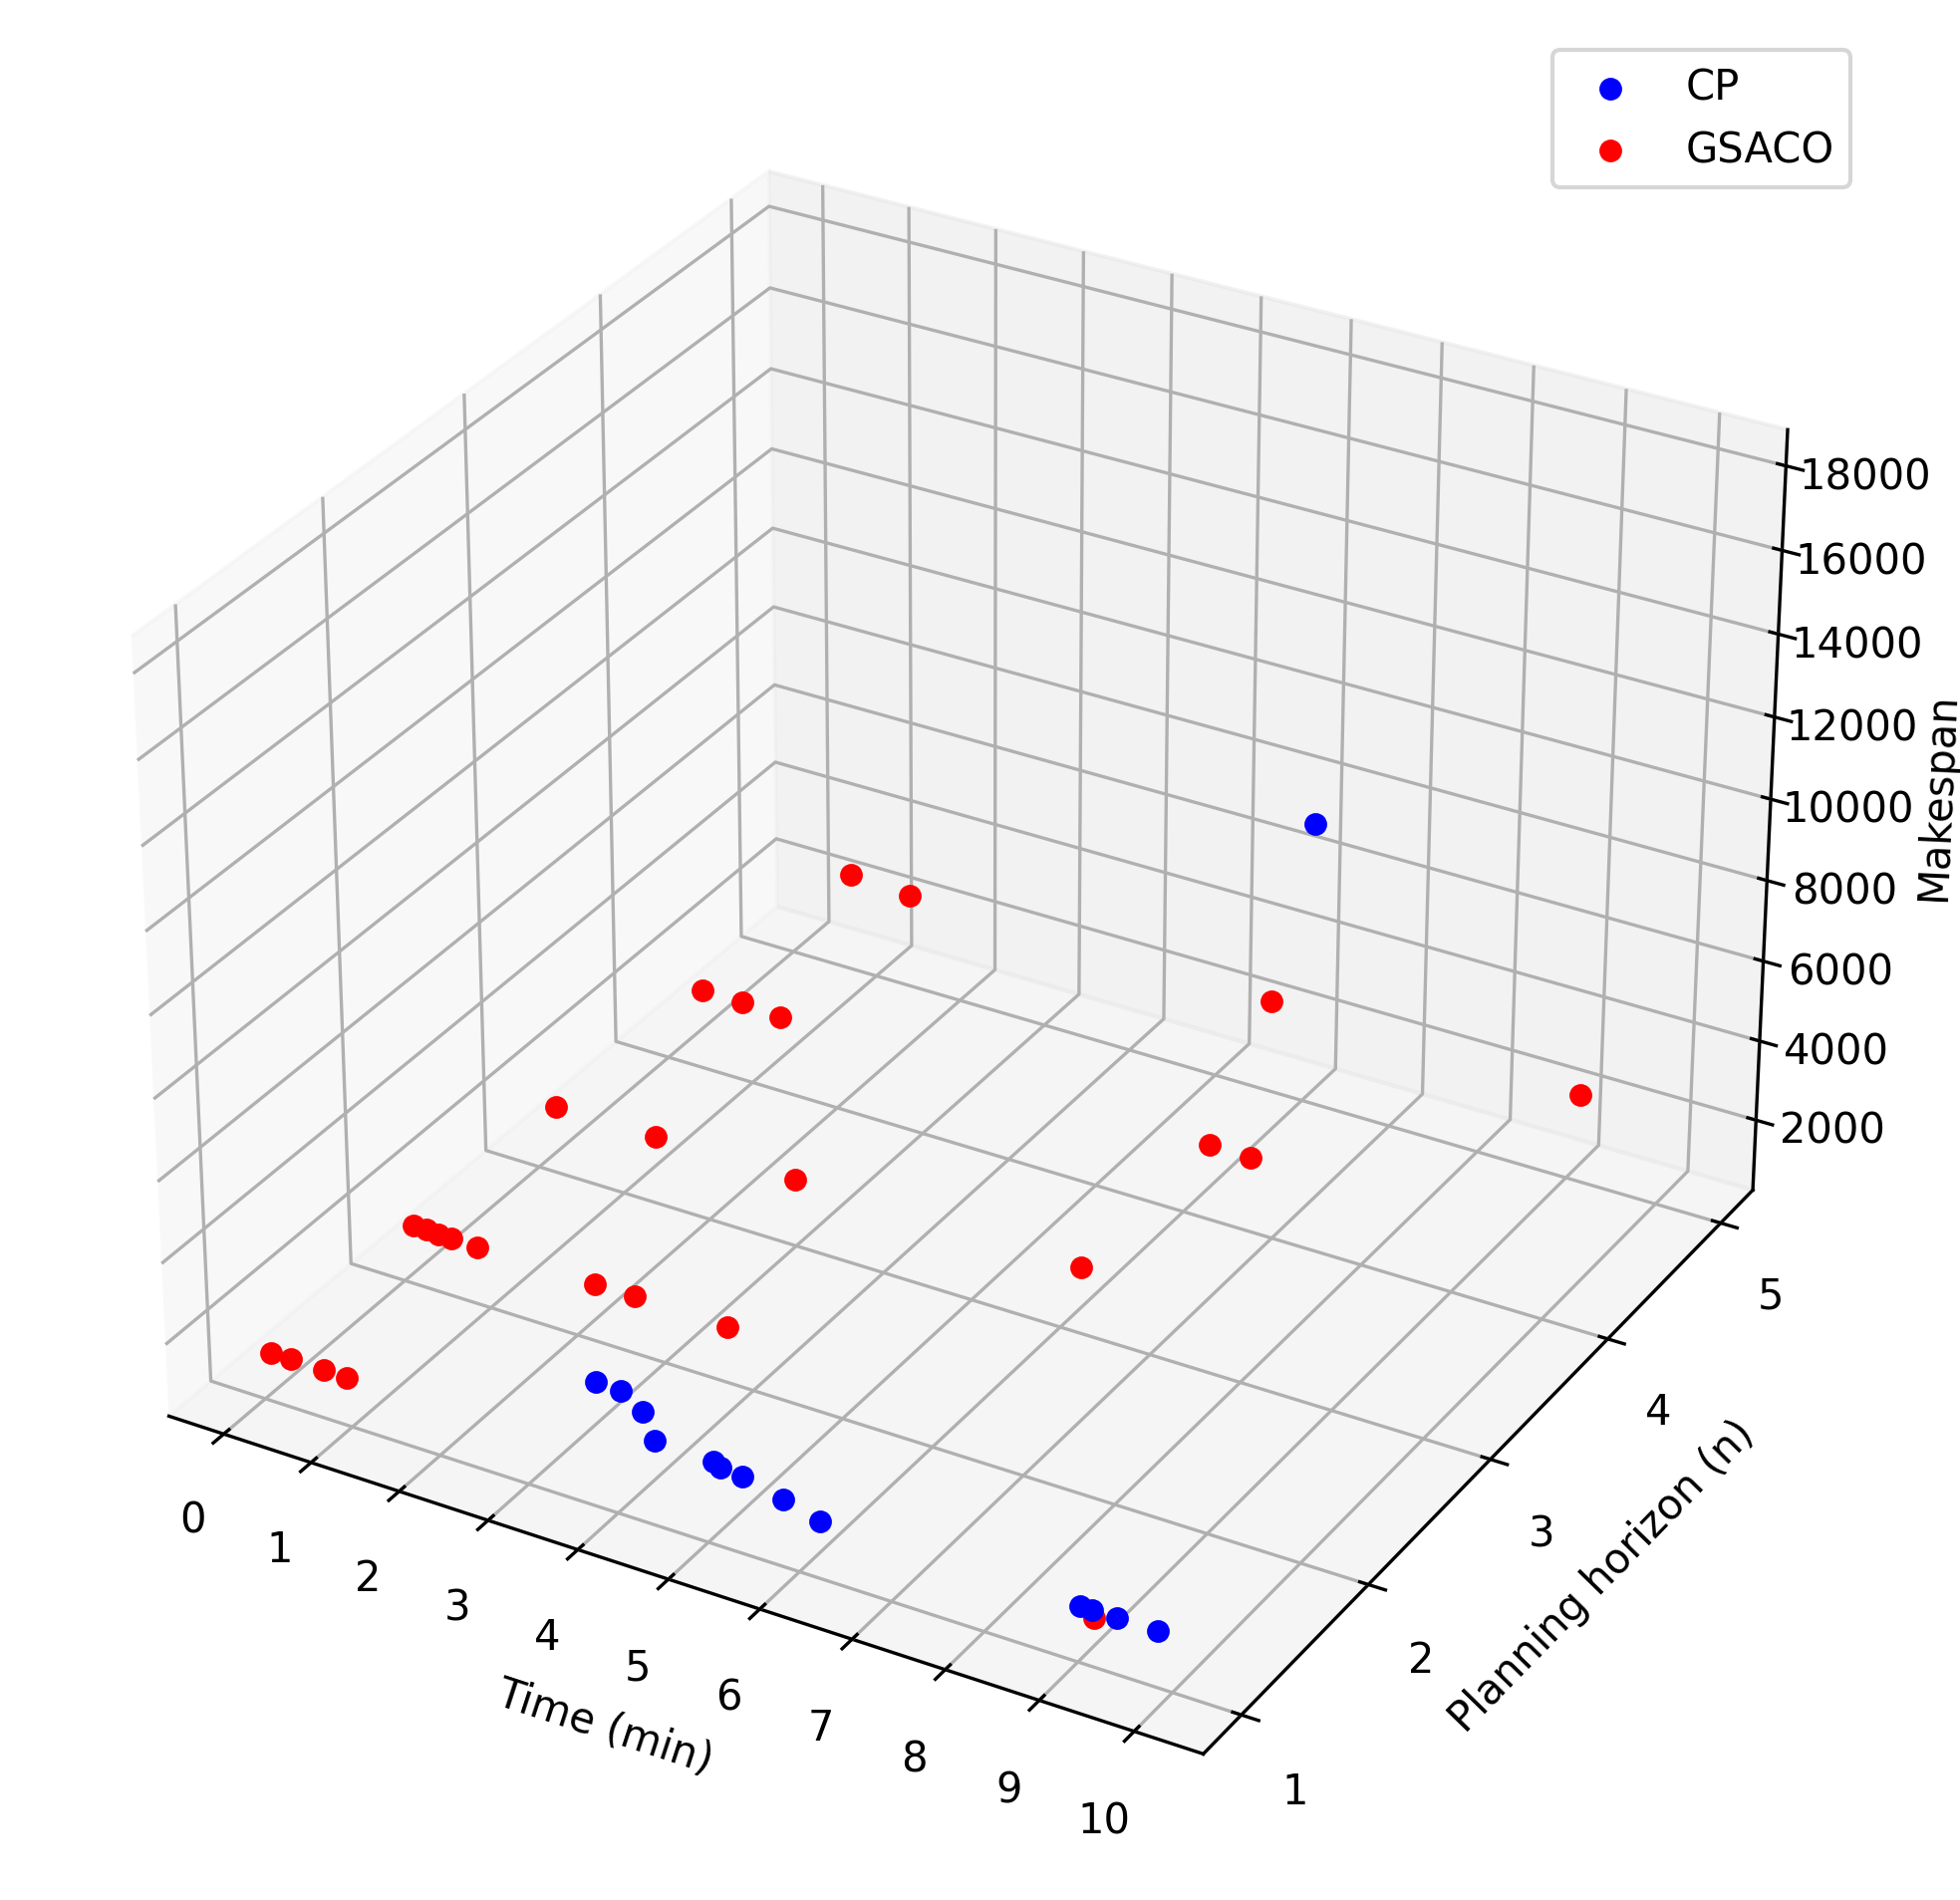
\includegraphics[width=\textwidth]{HVLM.png}
		\caption{HV/LM scenario}
		\label{subfig:h}
	\end{subfigure}
	\caption{Makespan improvements of schedules for SMSP instances obtained with CP and GSACO \cite{Ali2024}\label{fig:makespan}}
\end{figure*}

The quick convergence of our GSACO implementation is also outlined by the makespan improvements plotted in Figure~\ref{fig:makespan}.
On the LV/HM scenario displayed in Figure~\ref{subfig:l}, 
GSACO obtains its best schedules within $7$ minutes
for all planning horizons.
Only for the longest planning horizon $n=5$
on the HV/LM scenario in Figure~\ref{subfig:h},
an improvement occurs after more than the $9$ minutes of computing time
listed in the rightmost column of Table~\ref{tab:results}.
Comparing the SMSP instances for which OR-Tools manages to provide
feasible schedules,
the convergence to makespans in roughly the range of GSACO's results
takes significantly more computing time.
Hence, the time limit that would be necessary to break even with GSACO,
as accomplished within $7$ minutes for the shortest planning horizon
$n=1$ on the LV/HM scenario,
cannot be predicted for the SMSP instances with longer planning horizons.
Moreover, we observe that the initial schedules obtained 
in the first GSACO iteration by some of the ants running in parallel are of relatively high quality, while
OR-Tools sometimes finds outliers as its first solutions.
This phenomenon occurs for the planning horizons $n=1$ and $n=2$
on the LV/HM or HV/LM scenario, respectively, where the latter
schedule of makespan $17664$ is found after more than $9$ minutes
and thus not listed in Table~\ref{tab:results}.


\begin{table}[t]
	\caption{Comparative performance of dispatching strategies (LV/HM)}
	\label{tab:dispatchers-LVHM}
	\begin{tabular}{|c|lcllllll|ll|}
		\hline
		\multirow{3}{*}{\begin{tabular}[c]{@{}c@{}}Planning \\ horizon\end{tabular}} &
		\multicolumn{8}{c|}{Dispatcher} &
		\multicolumn{2}{c|}{Scheduler} \\ \cline{2-11} 
		&
		\multicolumn{2}{c|}{FIFO} &
		\multicolumn{2}{c|}{CR} &
		\multicolumn{2}{c|}{RANDOM} &
		\multicolumn{2}{c|}{GSACO-O} &
		\multicolumn{2}{c|}{GSACO-O} \\ \cline{2-11} 
		&
		\multicolumn{1}{l|}{Ops/Lots} &
		\multicolumn{1}{l|}{Diff} &
		\multicolumn{1}{l|}{Ops/Lots} &
		\multicolumn{1}{l|}{Diff} &
		\multicolumn{1}{l|}{Ops/Lots} &
		\multicolumn{1}{l|}{Diff} &
		\multicolumn{1}{l|}{Ops/Lots} &
		Diff &
		\multicolumn{1}{l|}{Ops/Lots} &
		diff \\ \hline
		1 &
		\multicolumn{1}{l|}{1419/0} &
		\multicolumn{1}{c|}{-} &
		\multicolumn{1}{l|}{1416/0} &
		\multicolumn{1}{l|}{-0.21\%} &
		\multicolumn{1}{l|}{1403/0} &
		\multicolumn{1}{l|}{-1.12\%} &
		\multicolumn{1}{l|}{1442//0} &
		1.62\% &
		\multicolumn{1}{l|}{1422/0} &
		0.21\% \\
		2 &
		\multicolumn{1}{l|}{2249/0} &
		\multicolumn{1}{c|}{-} &
		\multicolumn{1}{l|}{2328/0} &
		\multicolumn{1}{l|}{3.51\%} &
		\multicolumn{1}{l|}{2275/0} &
		\multicolumn{1}{l|}{1.15\%} &
		\multicolumn{1}{l|}{2409/0} &
		7.11\% &
		\multicolumn{1}{l|}{2368/0} &
		5.29\% \\
		3 &
		\multicolumn{1}{l|}{2384/0} &
		\multicolumn{1}{c|}{-} &
		\multicolumn{1}{l|}{3372/0} &
		\multicolumn{1}{l|}{2.67\%} &
		\multicolumn{1}{l|}{3314/0} &
		\multicolumn{1}{l|}{0.91\%} &
		\multicolumn{1}{l|}{3427/0} &
		4.35\% &
		\multicolumn{1}{l|}{3234/0} &
		-1.52\% \\
		4 &
		\multicolumn{1}{l|}{4018/1} &
		\multicolumn{1}{c|}{-} &
		\multicolumn{1}{l|}{4083/1} &
		\multicolumn{1}{l|}{1.61\%} &
		\multicolumn{1}{l|}{4039/1} &
		\multicolumn{1}{l|}{0.52\%} &
		\multicolumn{1}{l|}{4272/1} &
		6.32\% &
		\multicolumn{1}{l|}{4015/1} &
		-0.07\% \\
		5 &
		\multicolumn{1}{l|}{4901/1} &
		\multicolumn{1}{c|}{-} &
		\multicolumn{1}{l|}{5023/1} &
		\multicolumn{1}{l|}{2.48\%} &
		\multicolumn{1}{l|}{4972/1} &
		\multicolumn{1}{l|}{1.44\%} &
		\multicolumn{1}{l|}{5174/2} &
		5.57\% &
		\multicolumn{1}{l|}{4722/2} &
		-3.65\% \\
		6 &
		\multicolumn{1}{l|}{5665/4} &
		\multicolumn{1}{c|}{-} &
		\multicolumn{1}{l|}{5799/3} &
		\multicolumn{1}{l|}{2.36\%} &
		\multicolumn{1}{l|}{5767/1} &
		\multicolumn{1}{l|}{1.80\%} &
		\multicolumn{1}{l|}{6014/2} &
		6.16\% &
		\multicolumn{1}{l|}{5306/2} &
		-6.33\% \\ \hline
	\end{tabular}%
\end{table}

\begin{table}[t]
	\caption{Comparative performance of dispatching strategies (HV/LM)}
	\label{tab:dispatchers-HVLM}
	\begin{tabular}{|c|lcllllll|ll|}
		\hline
		\multirow{3}{*}{\begin{tabular}[c]{@{}c@{}}Planning \\ horizon\end{tabular}} &
		\multicolumn{8}{c|}{Disaptcher} &
		\multicolumn{2}{c|}{Scheduler} \\ \cline{2-11} 
		&
		\multicolumn{2}{c|}{FIFO} &
		\multicolumn{2}{c|}{CR} &
		\multicolumn{2}{c|}{RANDOM} &
		\multicolumn{2}{c|}{GSACO-O} &
		\multicolumn{2}{c|}{GSACO-O} \\ \cline{2-11} 
		&
		\multicolumn{1}{l|}{Ops/Lots} &
		\multicolumn{1}{l|}{Diff} &
		\multicolumn{1}{l|}{Ops/Lots} &
		\multicolumn{1}{l|}{Diff} &
		\multicolumn{1}{l|}{Ops/Lots} &
		\multicolumn{1}{l|}{Diff} &
		\multicolumn{1}{l|}{Ops/Lots} &
		Diff &
		\multicolumn{1}{l|}{Ops/Lots} &
		Diff \\ \hline
		1 &
		\multicolumn{1}{l|}{1821/0} &
		\multicolumn{1}{c|}{-} &
		\multicolumn{1}{l|}{1798/0} &
		\multicolumn{1}{l|}{-1.26\%} &
		\multicolumn{1}{l|}{1810/0} &
		\multicolumn{1}{l|}{-0.60\%} &
		\multicolumn{1}{l|}{1831/0} &
		0.54\% &
		\multicolumn{1}{l|}{1848/0} &
		1.48\% \\
		2 &
		\multicolumn{1}{l|}{2831/0} &
		\multicolumn{1}{c|}{-} &
		\multicolumn{1}{l|}{2811/0} &
		\multicolumn{1}{l|}{-0.71\%} &
		\multicolumn{1}{l|}{2852/0} &
		\multicolumn{1}{l|}{0.74\%} &
		\multicolumn{1}{l|}{2957/0} &
		4.45\% &
		\multicolumn{1}{l|}{2960/0} &
		4.55\% \\
		3 &
		\multicolumn{1}{l|}{4020/1} &
		\multicolumn{1}{c|}{-} &
		\multicolumn{1}{l|}{4021/1} &
		\multicolumn{1}{l|}{0.02\%} &
		\multicolumn{1}{l|}{4065/1} &
		\multicolumn{1}{l|}{1.12\%} &
		\multicolumn{1}{l|}{4162/1} &
		3.53\% &
		\multicolumn{1}{l|}{4093/1} &
		1.81\% \\
		4 &
		\multicolumn{1}{l|}{4914/4} &
		\multicolumn{1}{c|}{-} &
		\multicolumn{1}{l|}{4934/3} &
		\multicolumn{1}{l|}{0.40\%} &
		\multicolumn{1}{l|}{4975/3} &
		\multicolumn{1}{l|}{1.24\%} &
		\multicolumn{1}{l|}{5118/3} &
		4.15\% &
		\multicolumn{1}{l|}{4970/3} &
		1.07\% \\
		5 &
		\multicolumn{1}{l|}{5960/6} &
		\multicolumn{1}{c|}{-} &
		\multicolumn{1}{l|}{6003/5} &
		\multicolumn{1}{l|}{0.72\%} &
		\multicolumn{1}{l|}{6026/5} &
		\multicolumn{1}{l|}{1.10\%} &
		\multicolumn{1}{l|}{6263/5} &
		5.08\% &
		\multicolumn{1}{l|}{5975/5} &
		0.25\% \\
		6 &
		\multicolumn{1}{l|}{6841/8} &
		\multicolumn{1}{c|}{-} &
		\multicolumn{1}{l|}{6946/8} &
		\multicolumn{1}{l|}{1.53\%} &
		\multicolumn{1}{l|}{6973/9} &
		\multicolumn{1}{l|}{1.92\%} &
		\multicolumn{1}{l|}{7162/7} &
		4.69\% &
		\multicolumn{1}{l|}{6716/7} &
		-1.82\% \\ \hline
	\end{tabular}%
\end{table}

Furthermore, this study investigates the efficiency of various dispatching strategies in a simulated manufacturing environment. Dispatchers play a critical role in production systems by determining the order in which jobs are processed. Effective dispatching can significantly enhance operational throughput and resource utilization. To this end, we compare traditional and enhanced dispatching based on a GSACO-O. The primary objective is to quantify and compare the performance changes of different dispatching strategies over multiple planning horizons.

We examined the efficacy of four distinct dispatching strategies using two different datasets, characterized as High Volume Low Mix (HV/LM) and Low Volume High Mix (LV/HM), to evaluate their effectiveness across six varied planning horizons. The strategies examined included First In, First Out (FIFO), Critical Ratio (CR), Random (RANDOM), and a Greedy Search based Ant Colony Optimization variant (GSACO-O), which is also assessed as a scheduler. The performance metrics were recorded in terms of operations and lots completed, with FIFO serving as the baseline for performance comparison.

The results from the LV/HM dataset shown in Table~\ref{tab:dispatchers-LVHM} indicate variable performance across the strategies and horizons. FIFO maintained consistent throughput but was generally outperformed by our GSACO-O dispatcher, which showed substantial increases in operational efficiency. Similarly, the results from HV/LM dataset shown in Table~\ref{tab:dispatchers-HVLM} further substantiate the superior performance of the GSACO-O strategy, confirming its effectiveness across different planning horizons.

The poor performance of GSACO-O over long planning horizon, as a scheduler compared to its role as a dispatcher can be attributed to the operational complexities. While dispatching focuses on immediate, localized decision-making related to the sequence and priority of jobs within the manufacturing process, scheduling involves long-term planning, requiring the management of more complex variables over extended periods. The GSACO-O algorithm, which combines greedy search and swarm intelligence, excels in environments where data is abundant and immediate adaptability is crucial, making it highly effective for dispatching. However, as a scheduler, the algorithm must contend with uncertainties such as fluctuating future orders and resource availability, which may not be as predictable as the current operational statuses utilized in dispatching. Moreover, the effectiveness of a scheduler is often gauged on long-term outcomes such as overall resource utilization and job load balancing, metrics that require a different approach or algorithmic tuning than those used for dispatching tasks.

\begin{figure}[t]
	\centering
	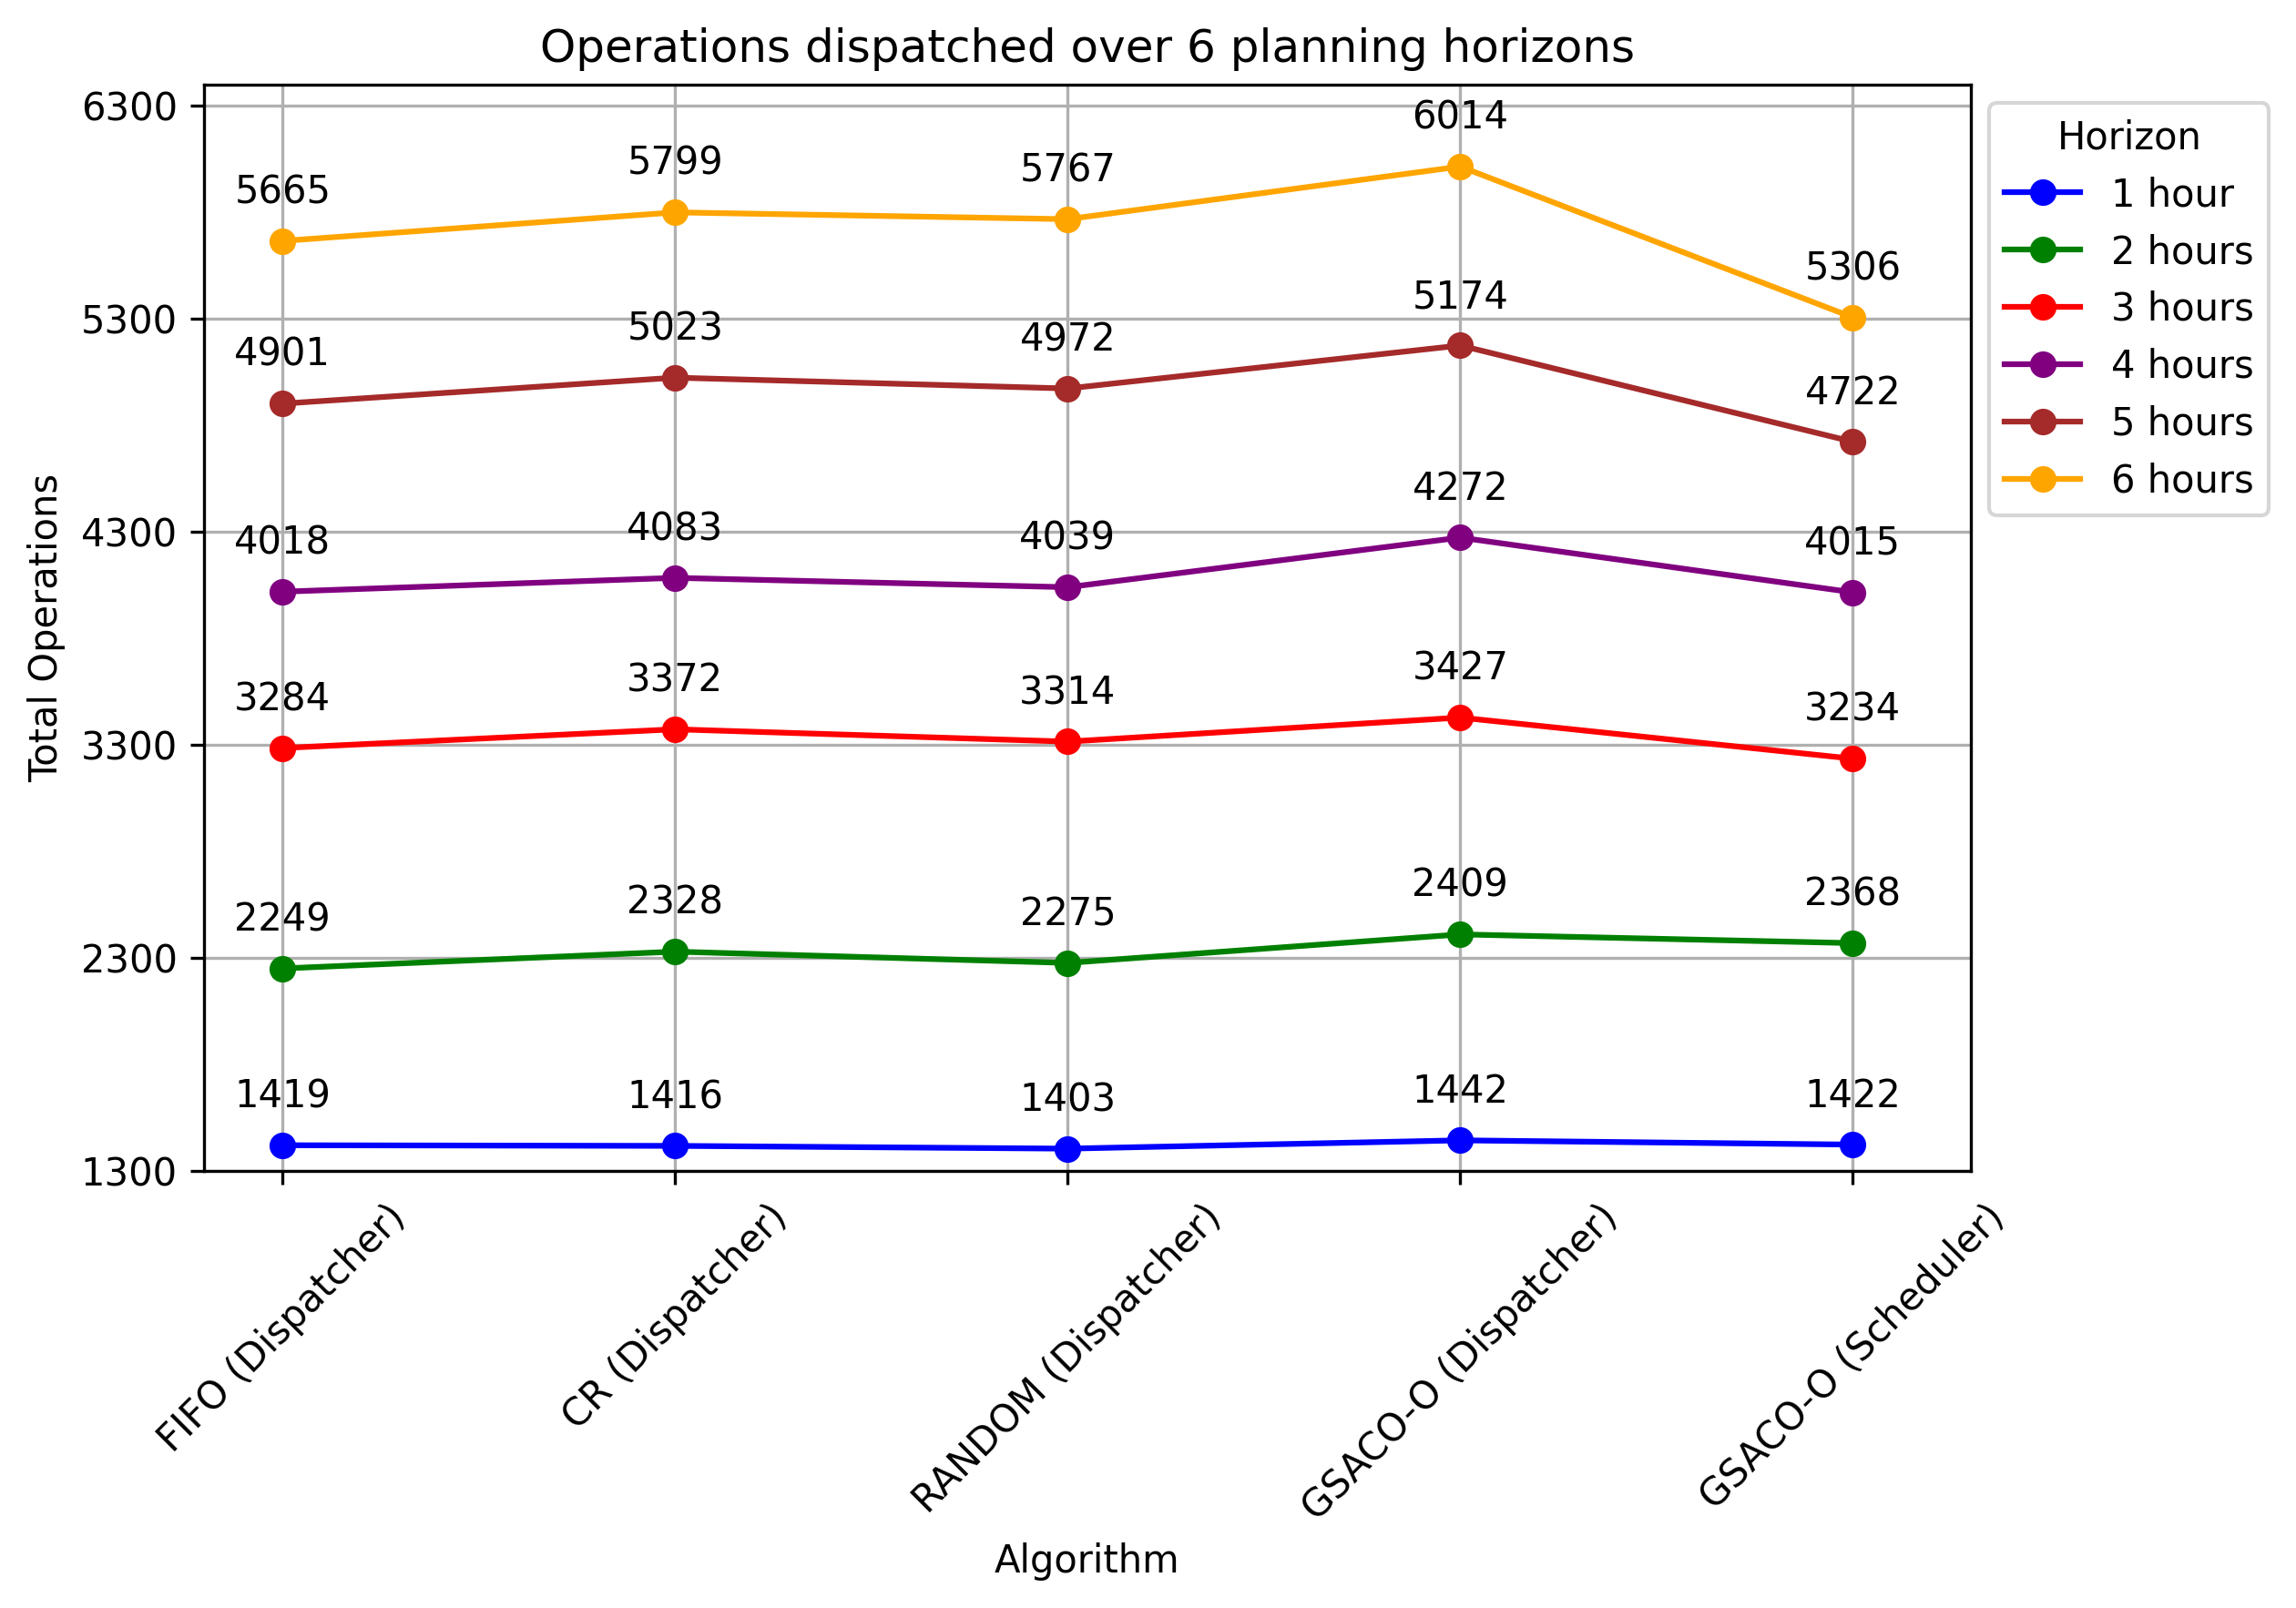
\includegraphics[width=\textwidth]{LVHM/operations_LVHM.png}
	\caption{Operations throughput (LV/HM)}
	\label{fig:totalopsLVHM}
\end{figure}

\begin{figure}[t]
	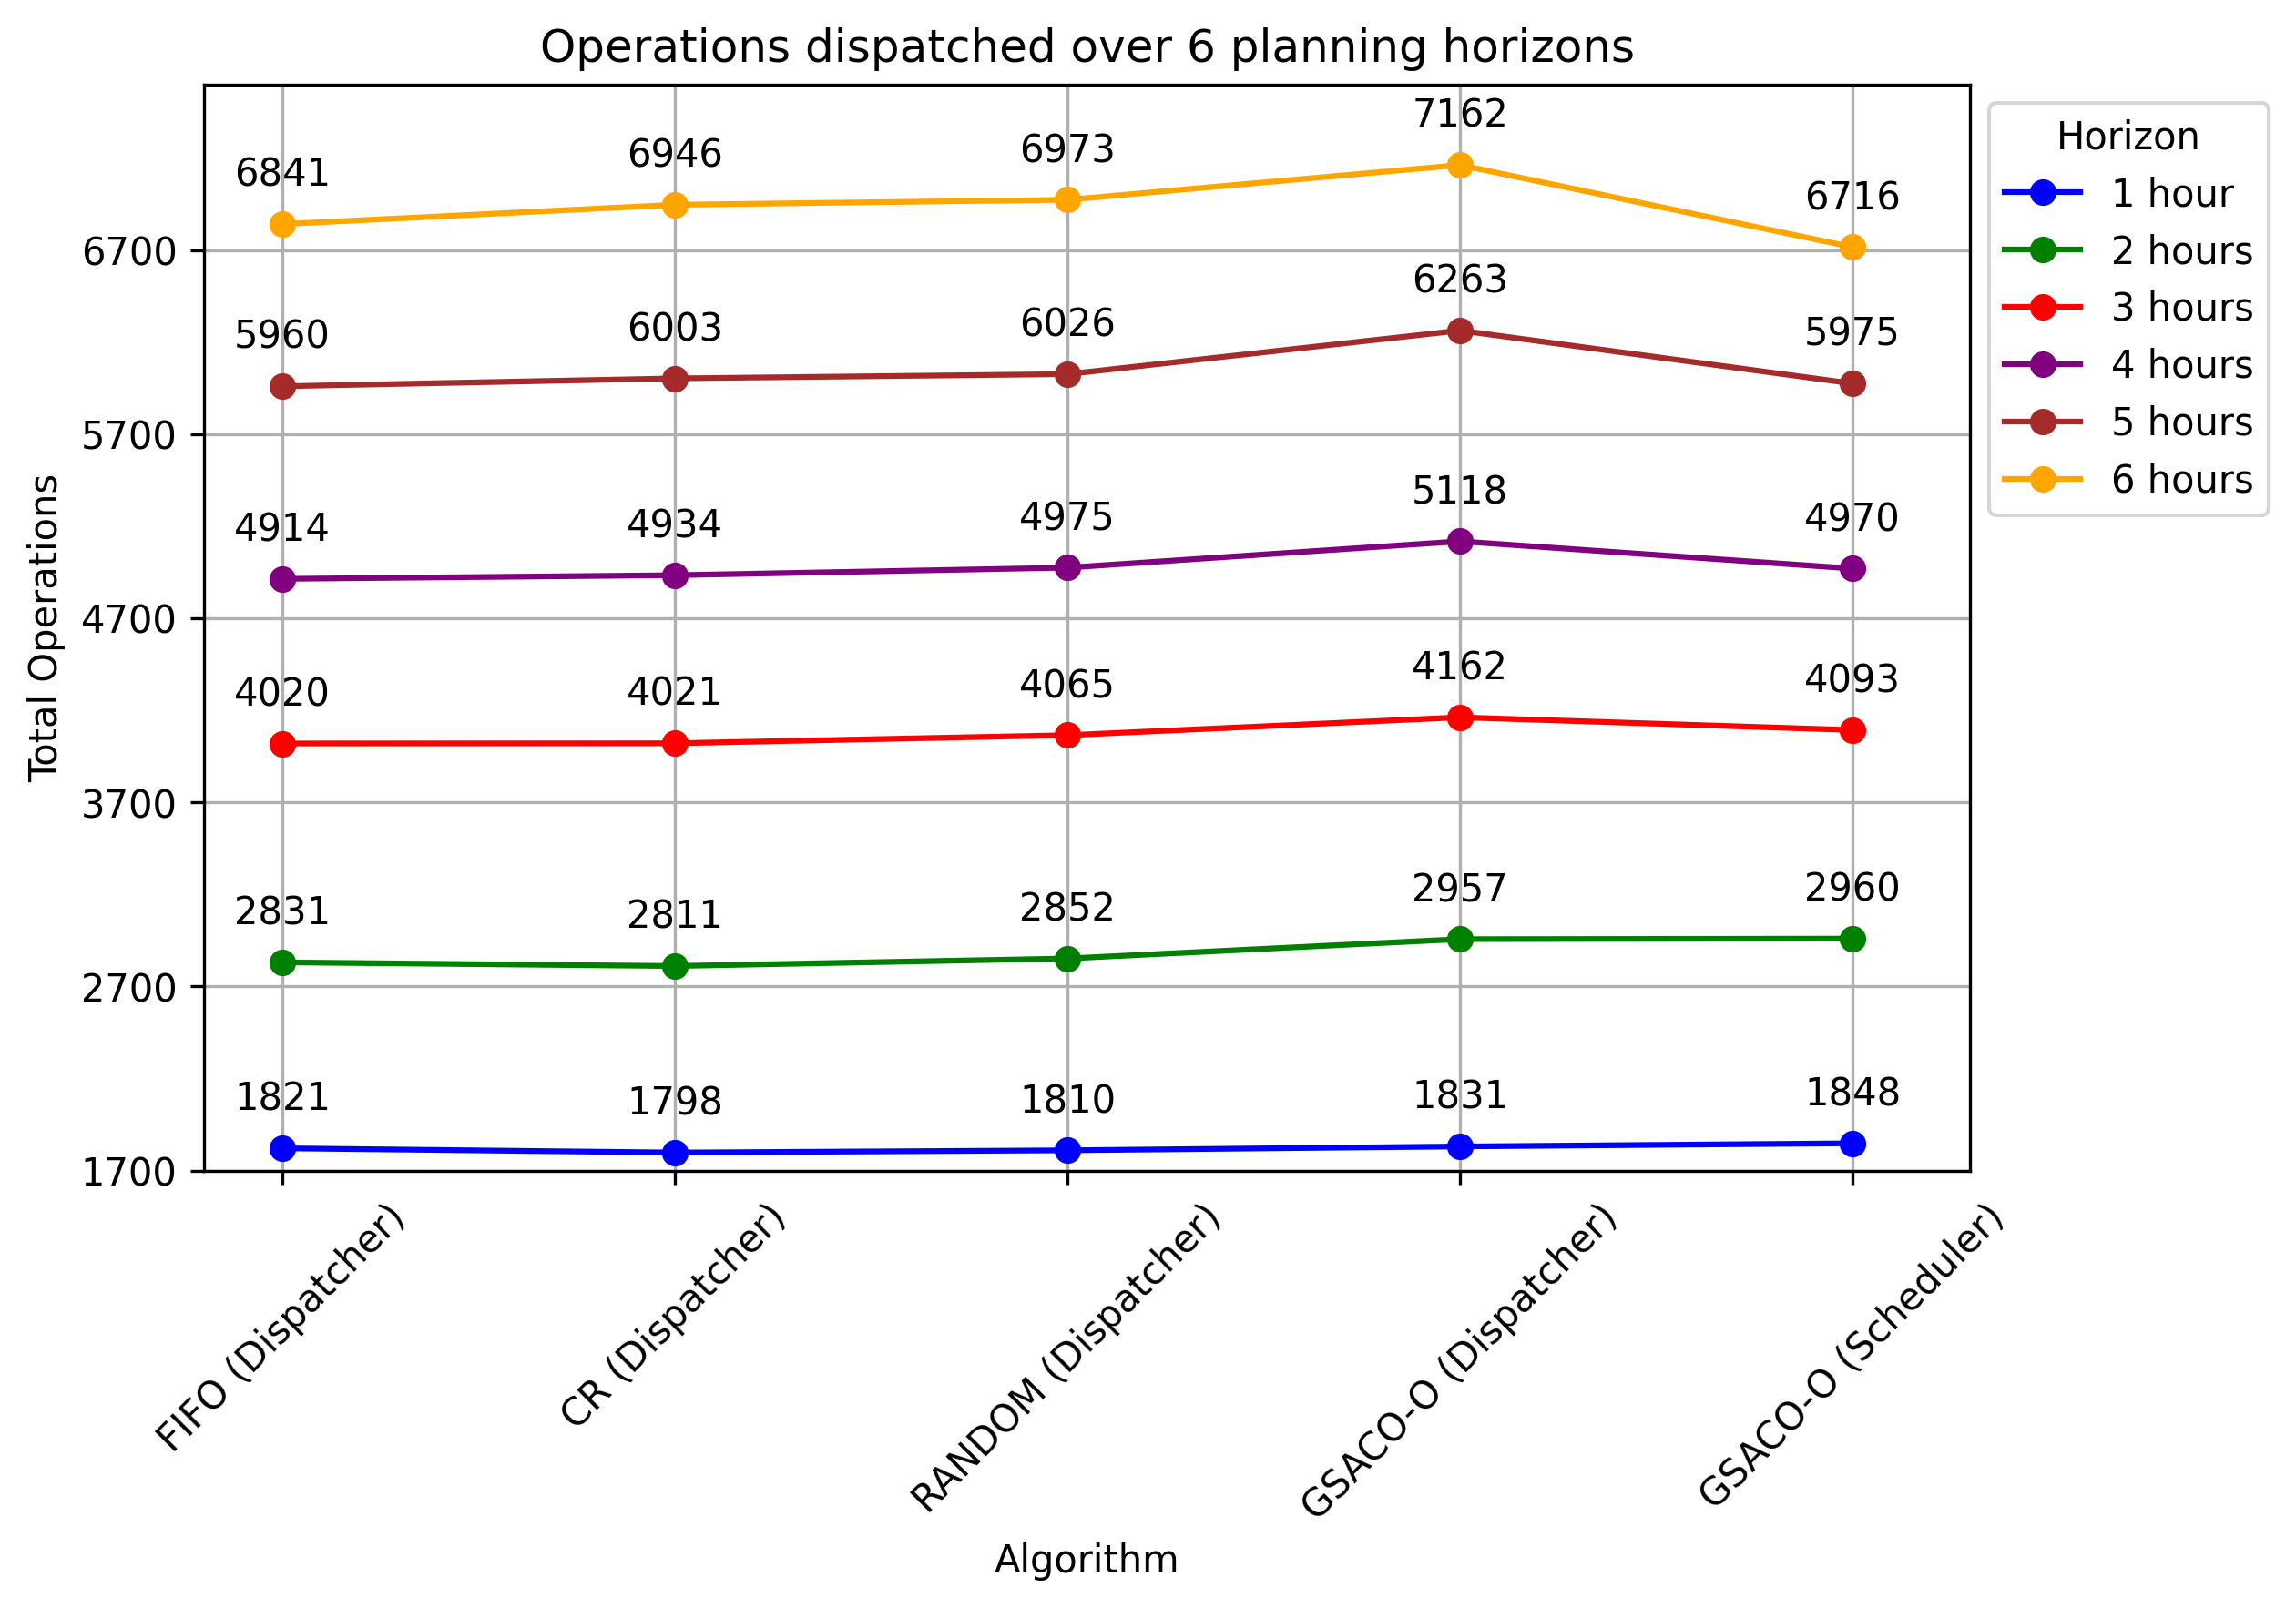
\includegraphics[width=\textwidth]{HVLM/operations_HVLM.png}
	\caption{Operations throughput (HV/LM)}
	\label{fig:totalopsHVLM}
\end{figure}

In Figure~\ref{fig:totalopsLVHM} and Figure~\ref{fig:totalopsHVLM}, the performance of dispatching rules; FIFO, CR, RANDOM, GSACO-O and GSACO-O as scheduler across different planning horizons ranging from 1 to 6 hours is presented. Each plot illustrates the total number of operations dispatched by each rule within these time frames, offering a clear comparison of their efficiency and effectiveness in handling operational tasks within a semiconductor manufacturing.


\begin{figure}[t]
	\centering
	\begin{subfigure}{0.32\textwidth}
		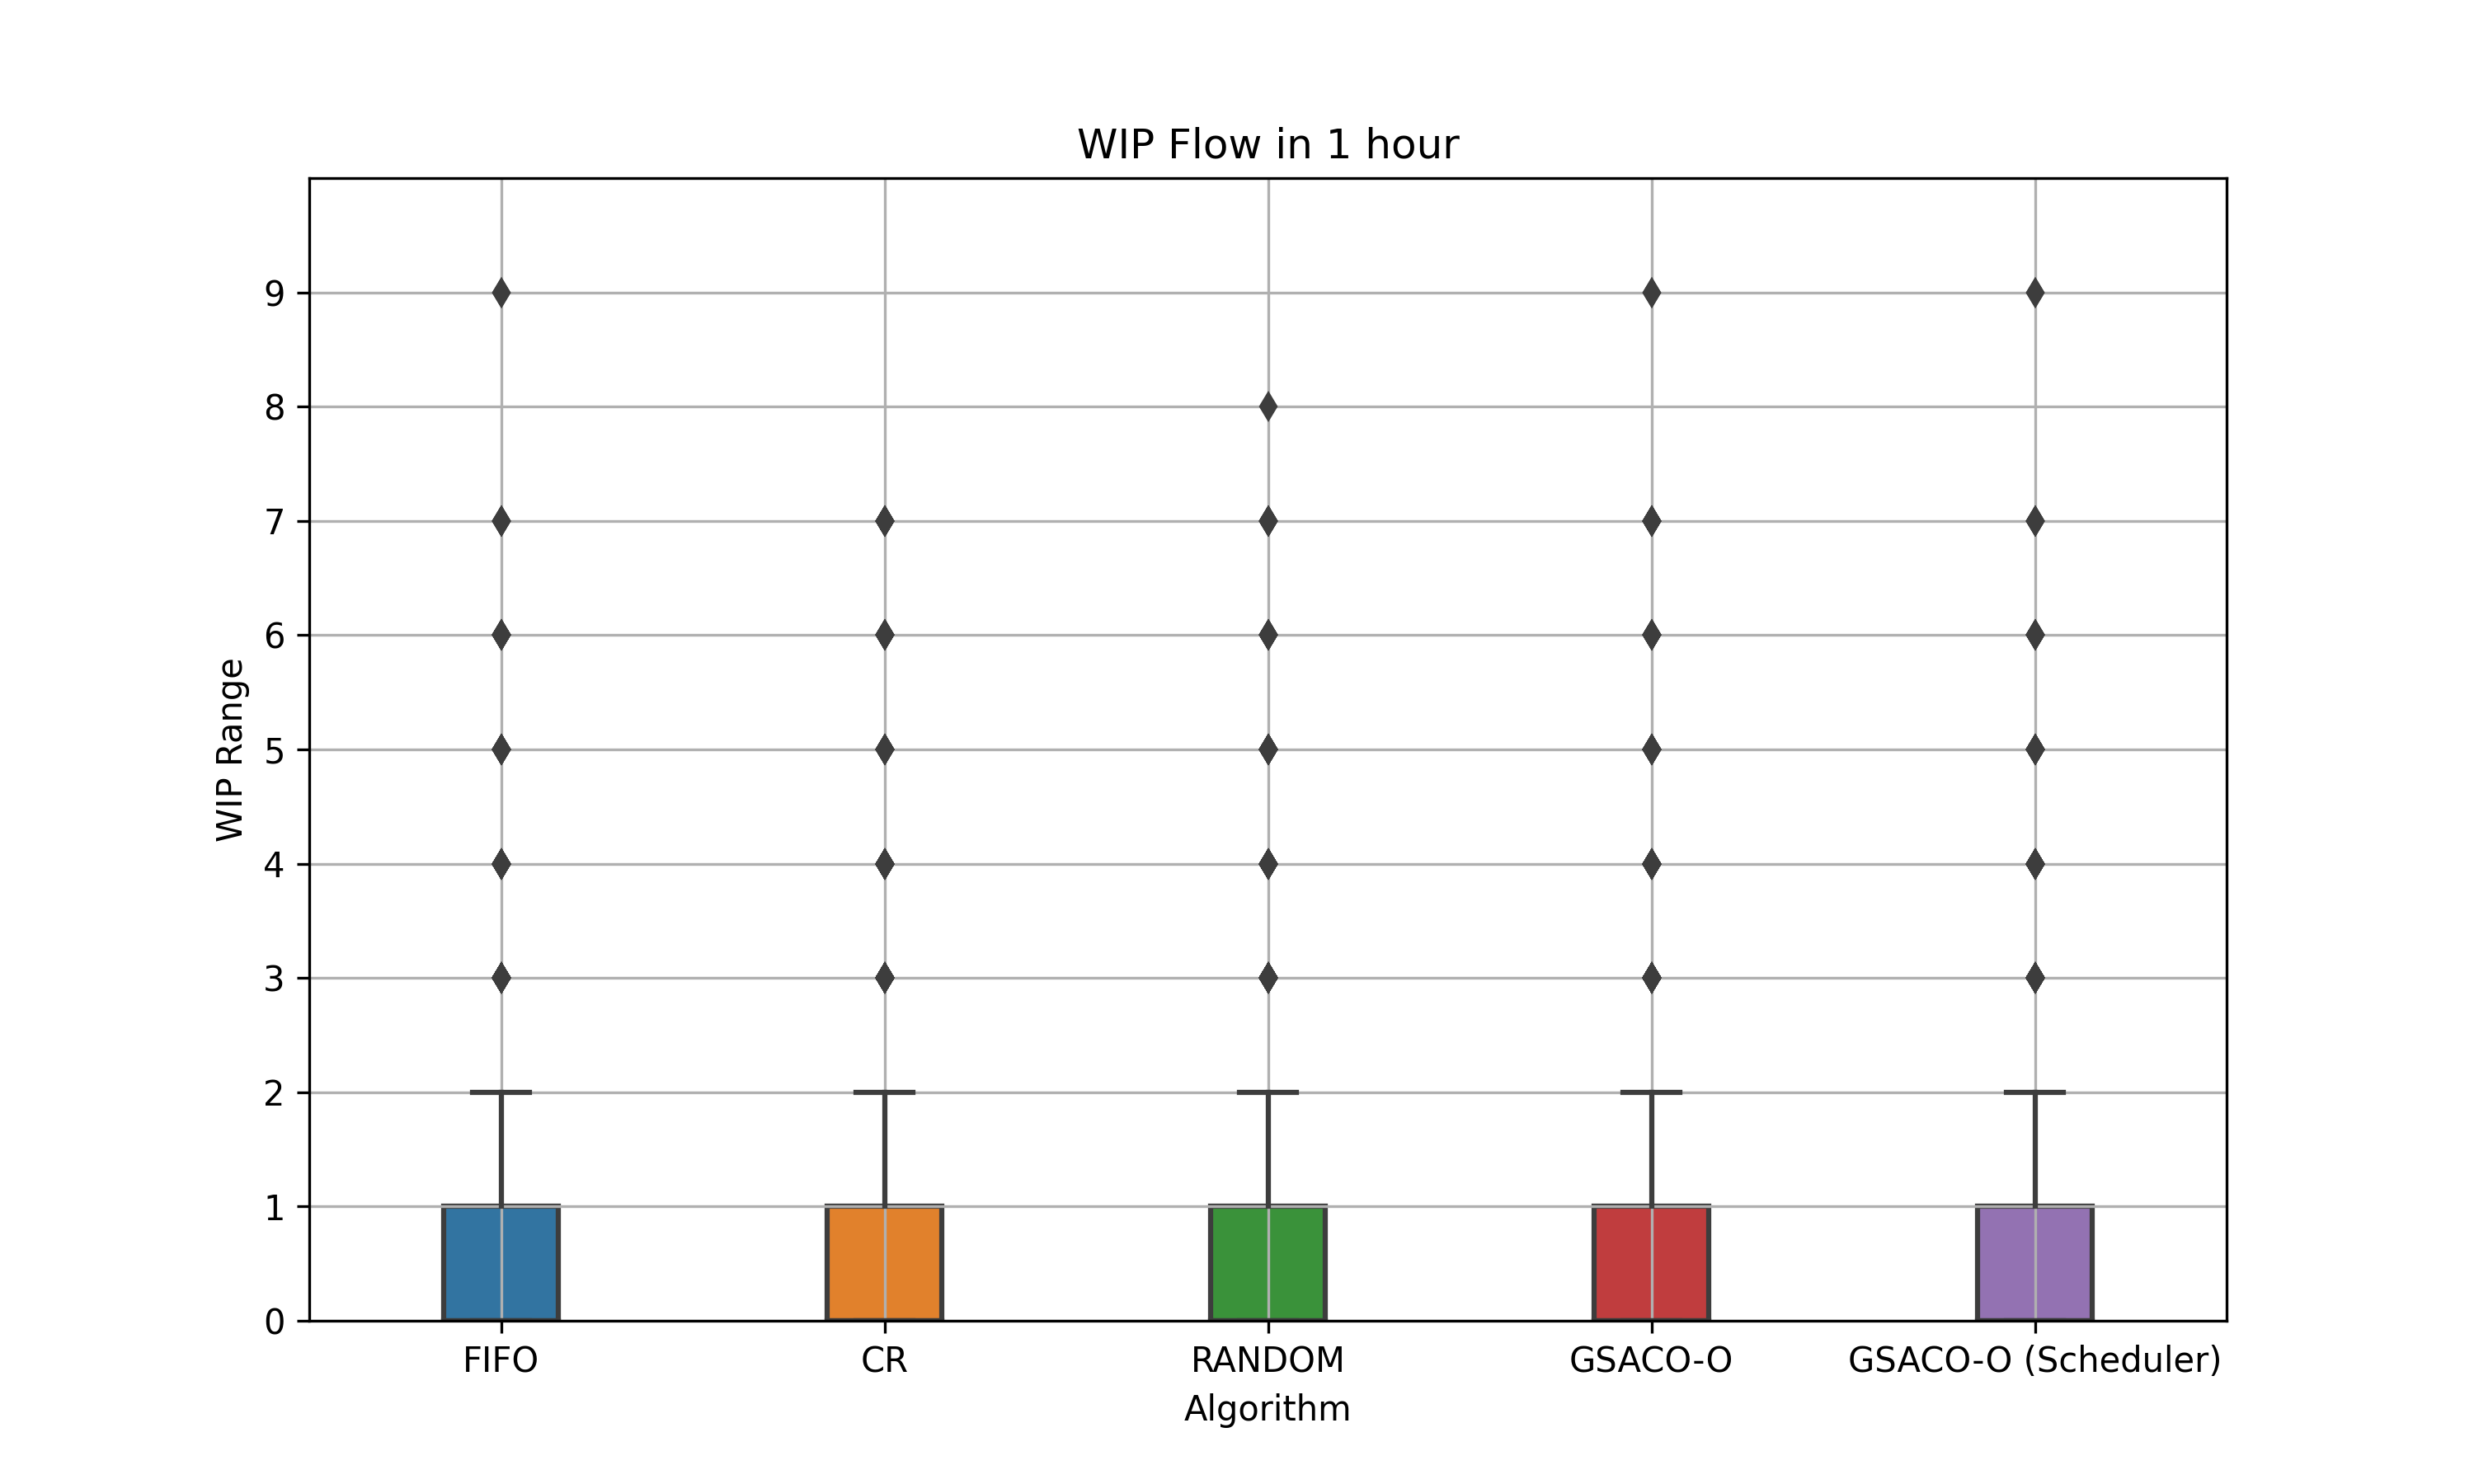
\includegraphics[width=\textwidth]{LVHM/new_period_3600s.png}
		% \caption{}
		% \label{fig:pp1}
	\end{subfigure}\hfill
	\begin{subfigure}{0.32\textwidth}
		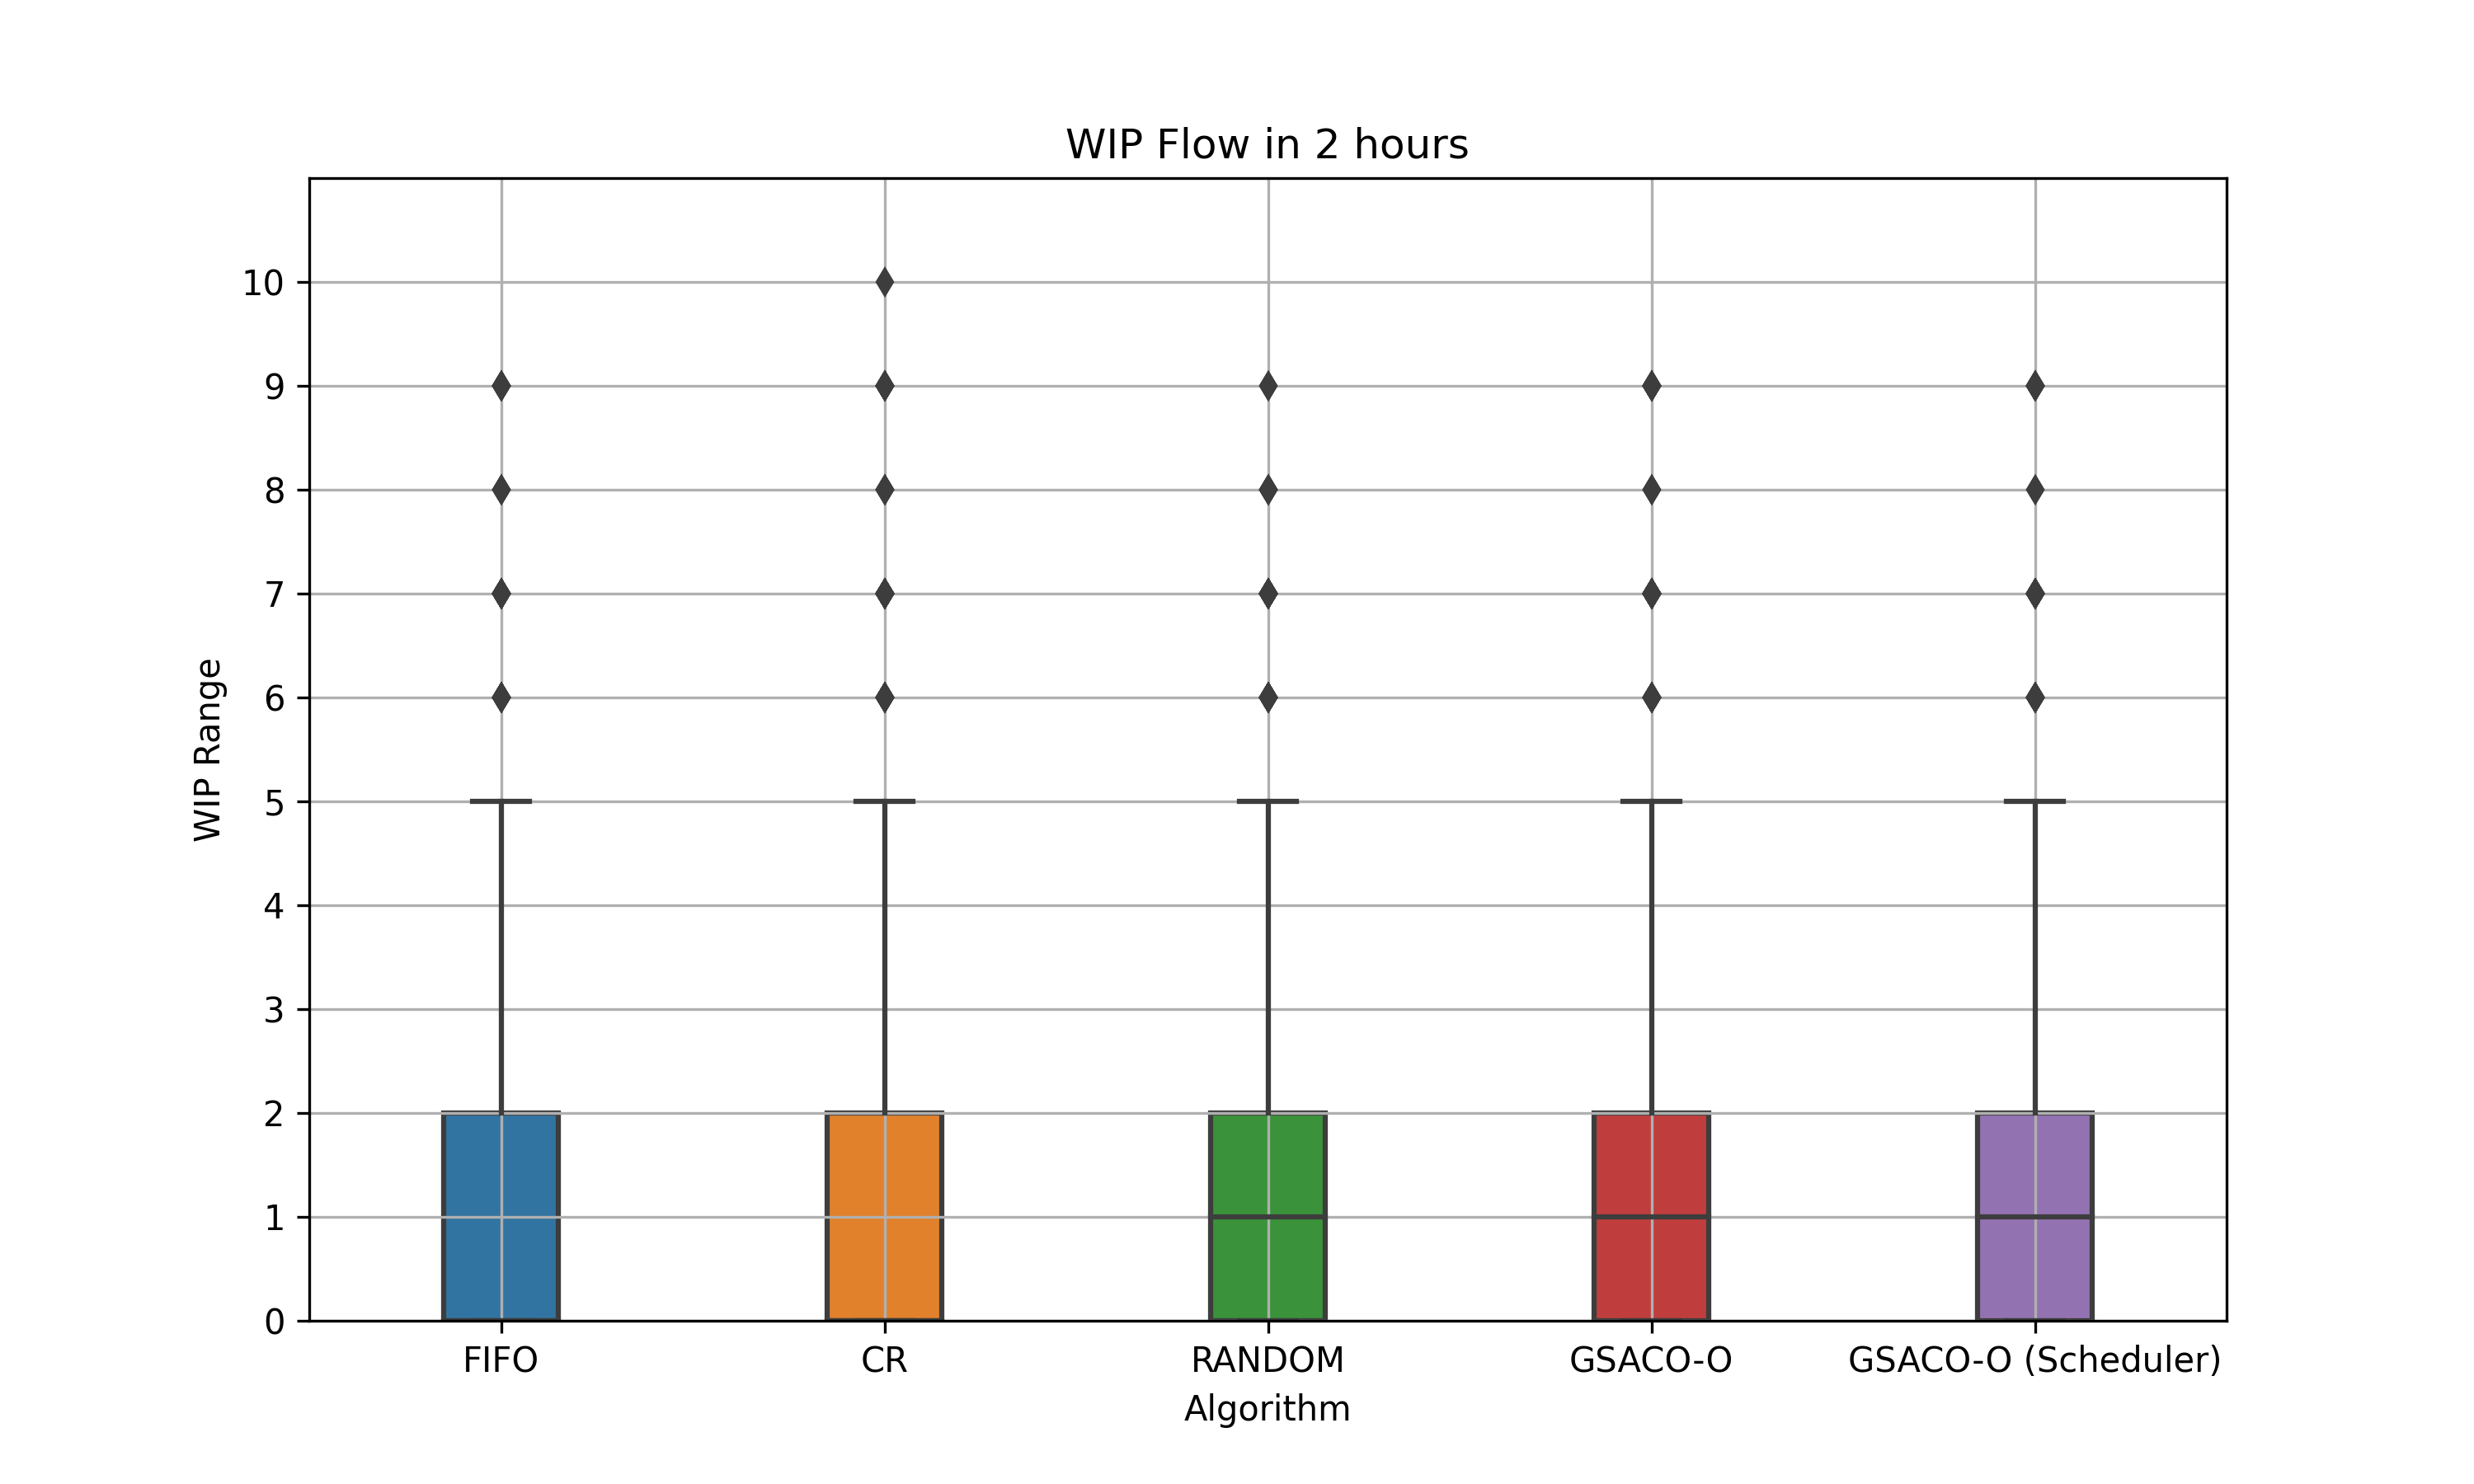
\includegraphics[width=\textwidth]{LVHM/new_period_7200s.png}
		% \caption{}
		% \label{fig:pp2}
	\end{subfigure}\hfill
	\begin{subfigure}{0.32\textwidth}
		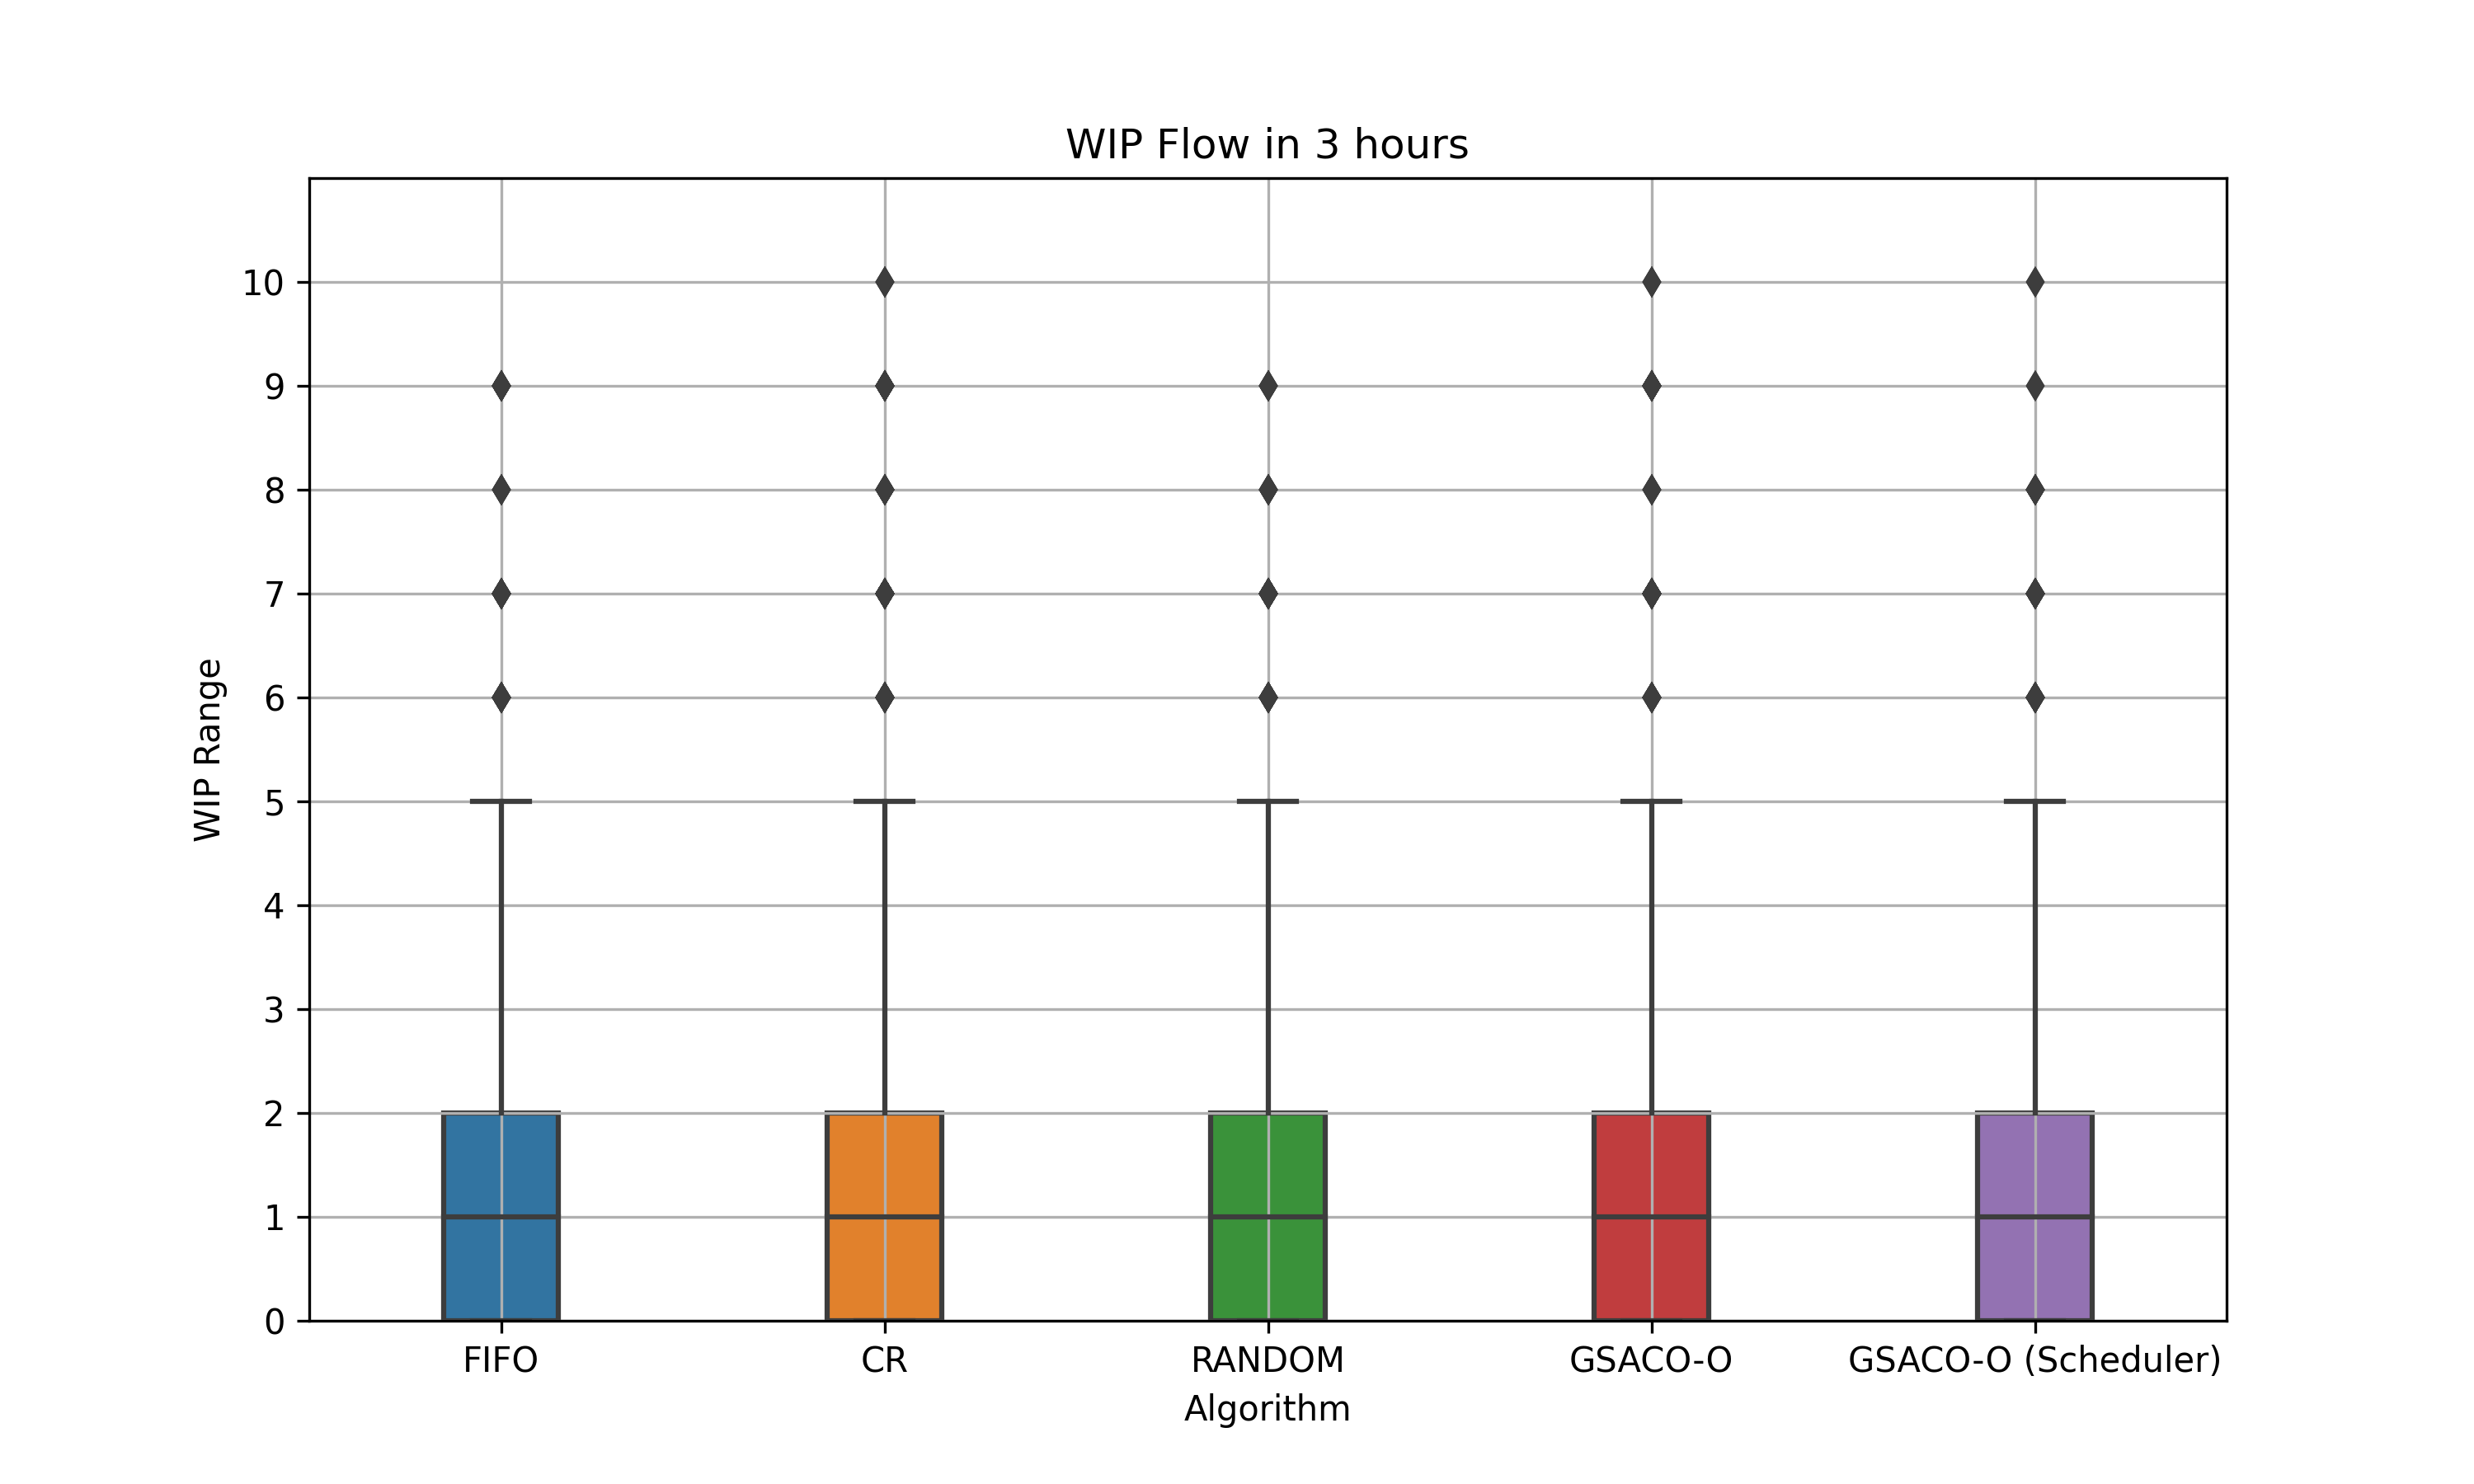
\includegraphics[width=\textwidth]{LVHM/new_period_10800s.png}
		% \caption{}
		% \label{fig:pp3}
	\end{subfigure}
	\begin{subfigure}{0.32\textwidth}
		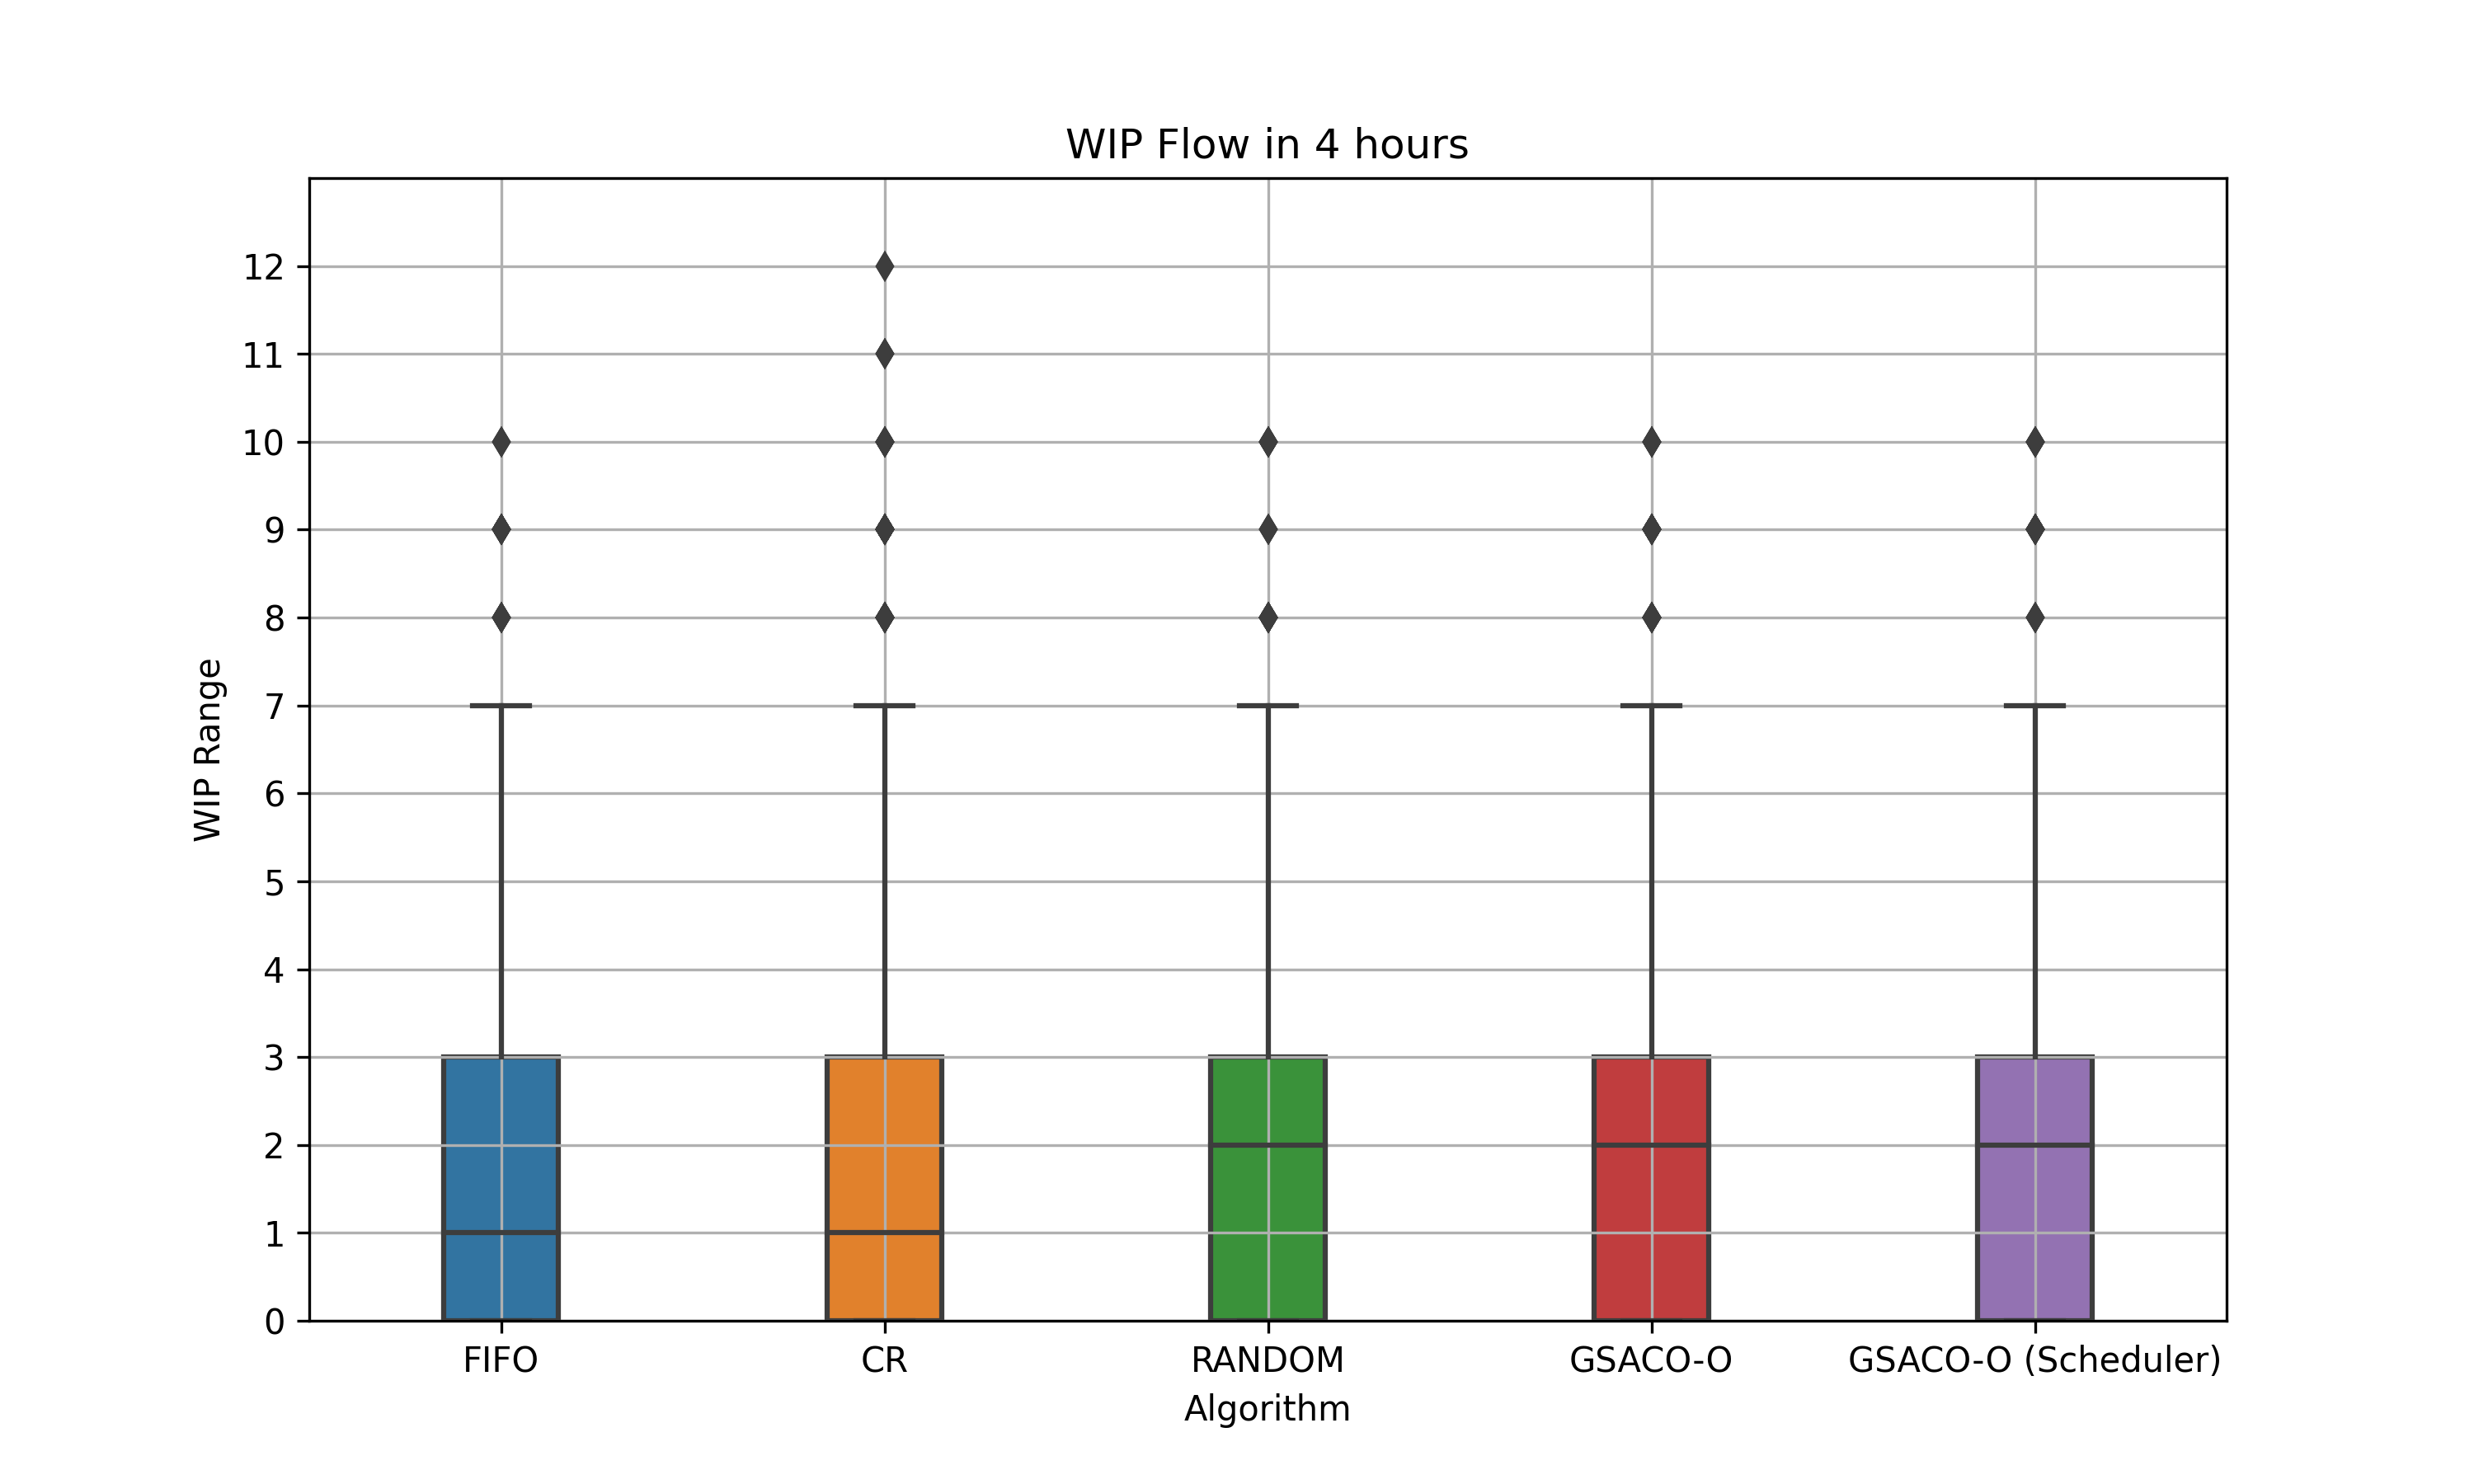
\includegraphics[width=\textwidth]{LVHM/new_period_14400s.png}
		% \caption{}
		% \label{fig:pp4}
	\end{subfigure}\hfill
	\begin{subfigure}{0.32\textwidth}
		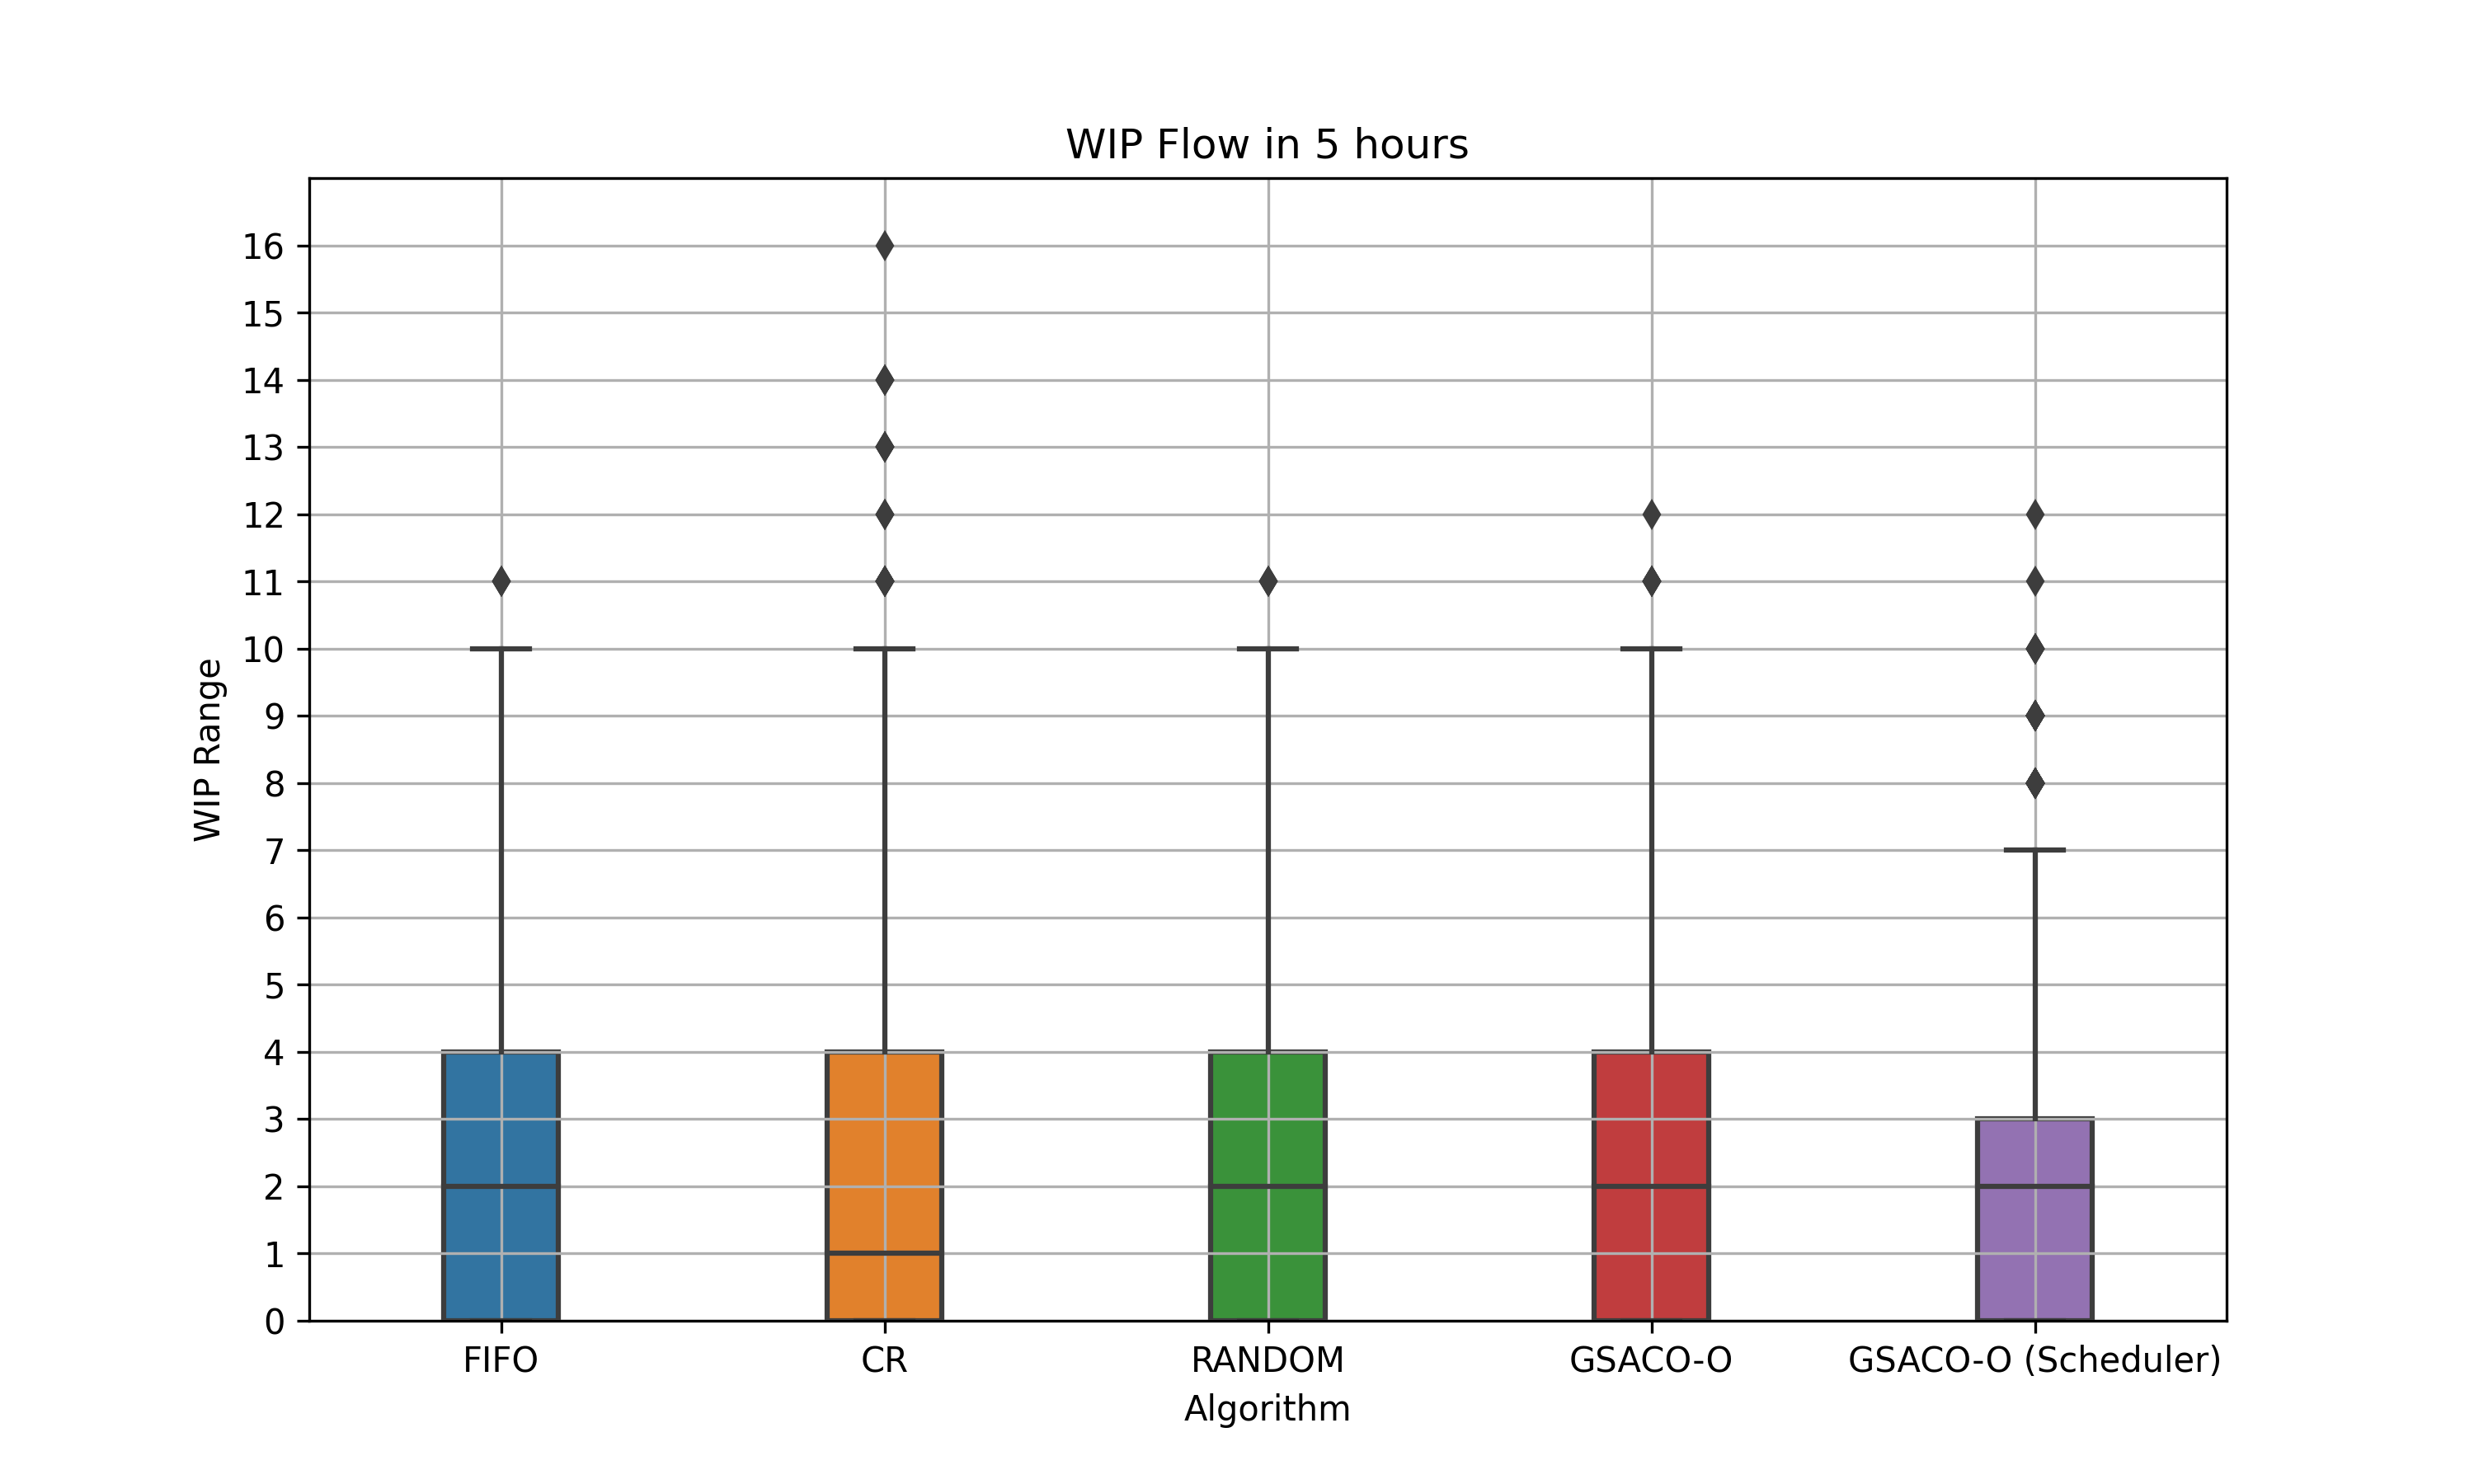
\includegraphics[width=\textwidth]{LVHM/new_period_18000s.png}
		% \caption{}
		% \label{fig:pp5}
	\end{subfigure}\hfill
	\begin{subfigure}{0.32\textwidth}
		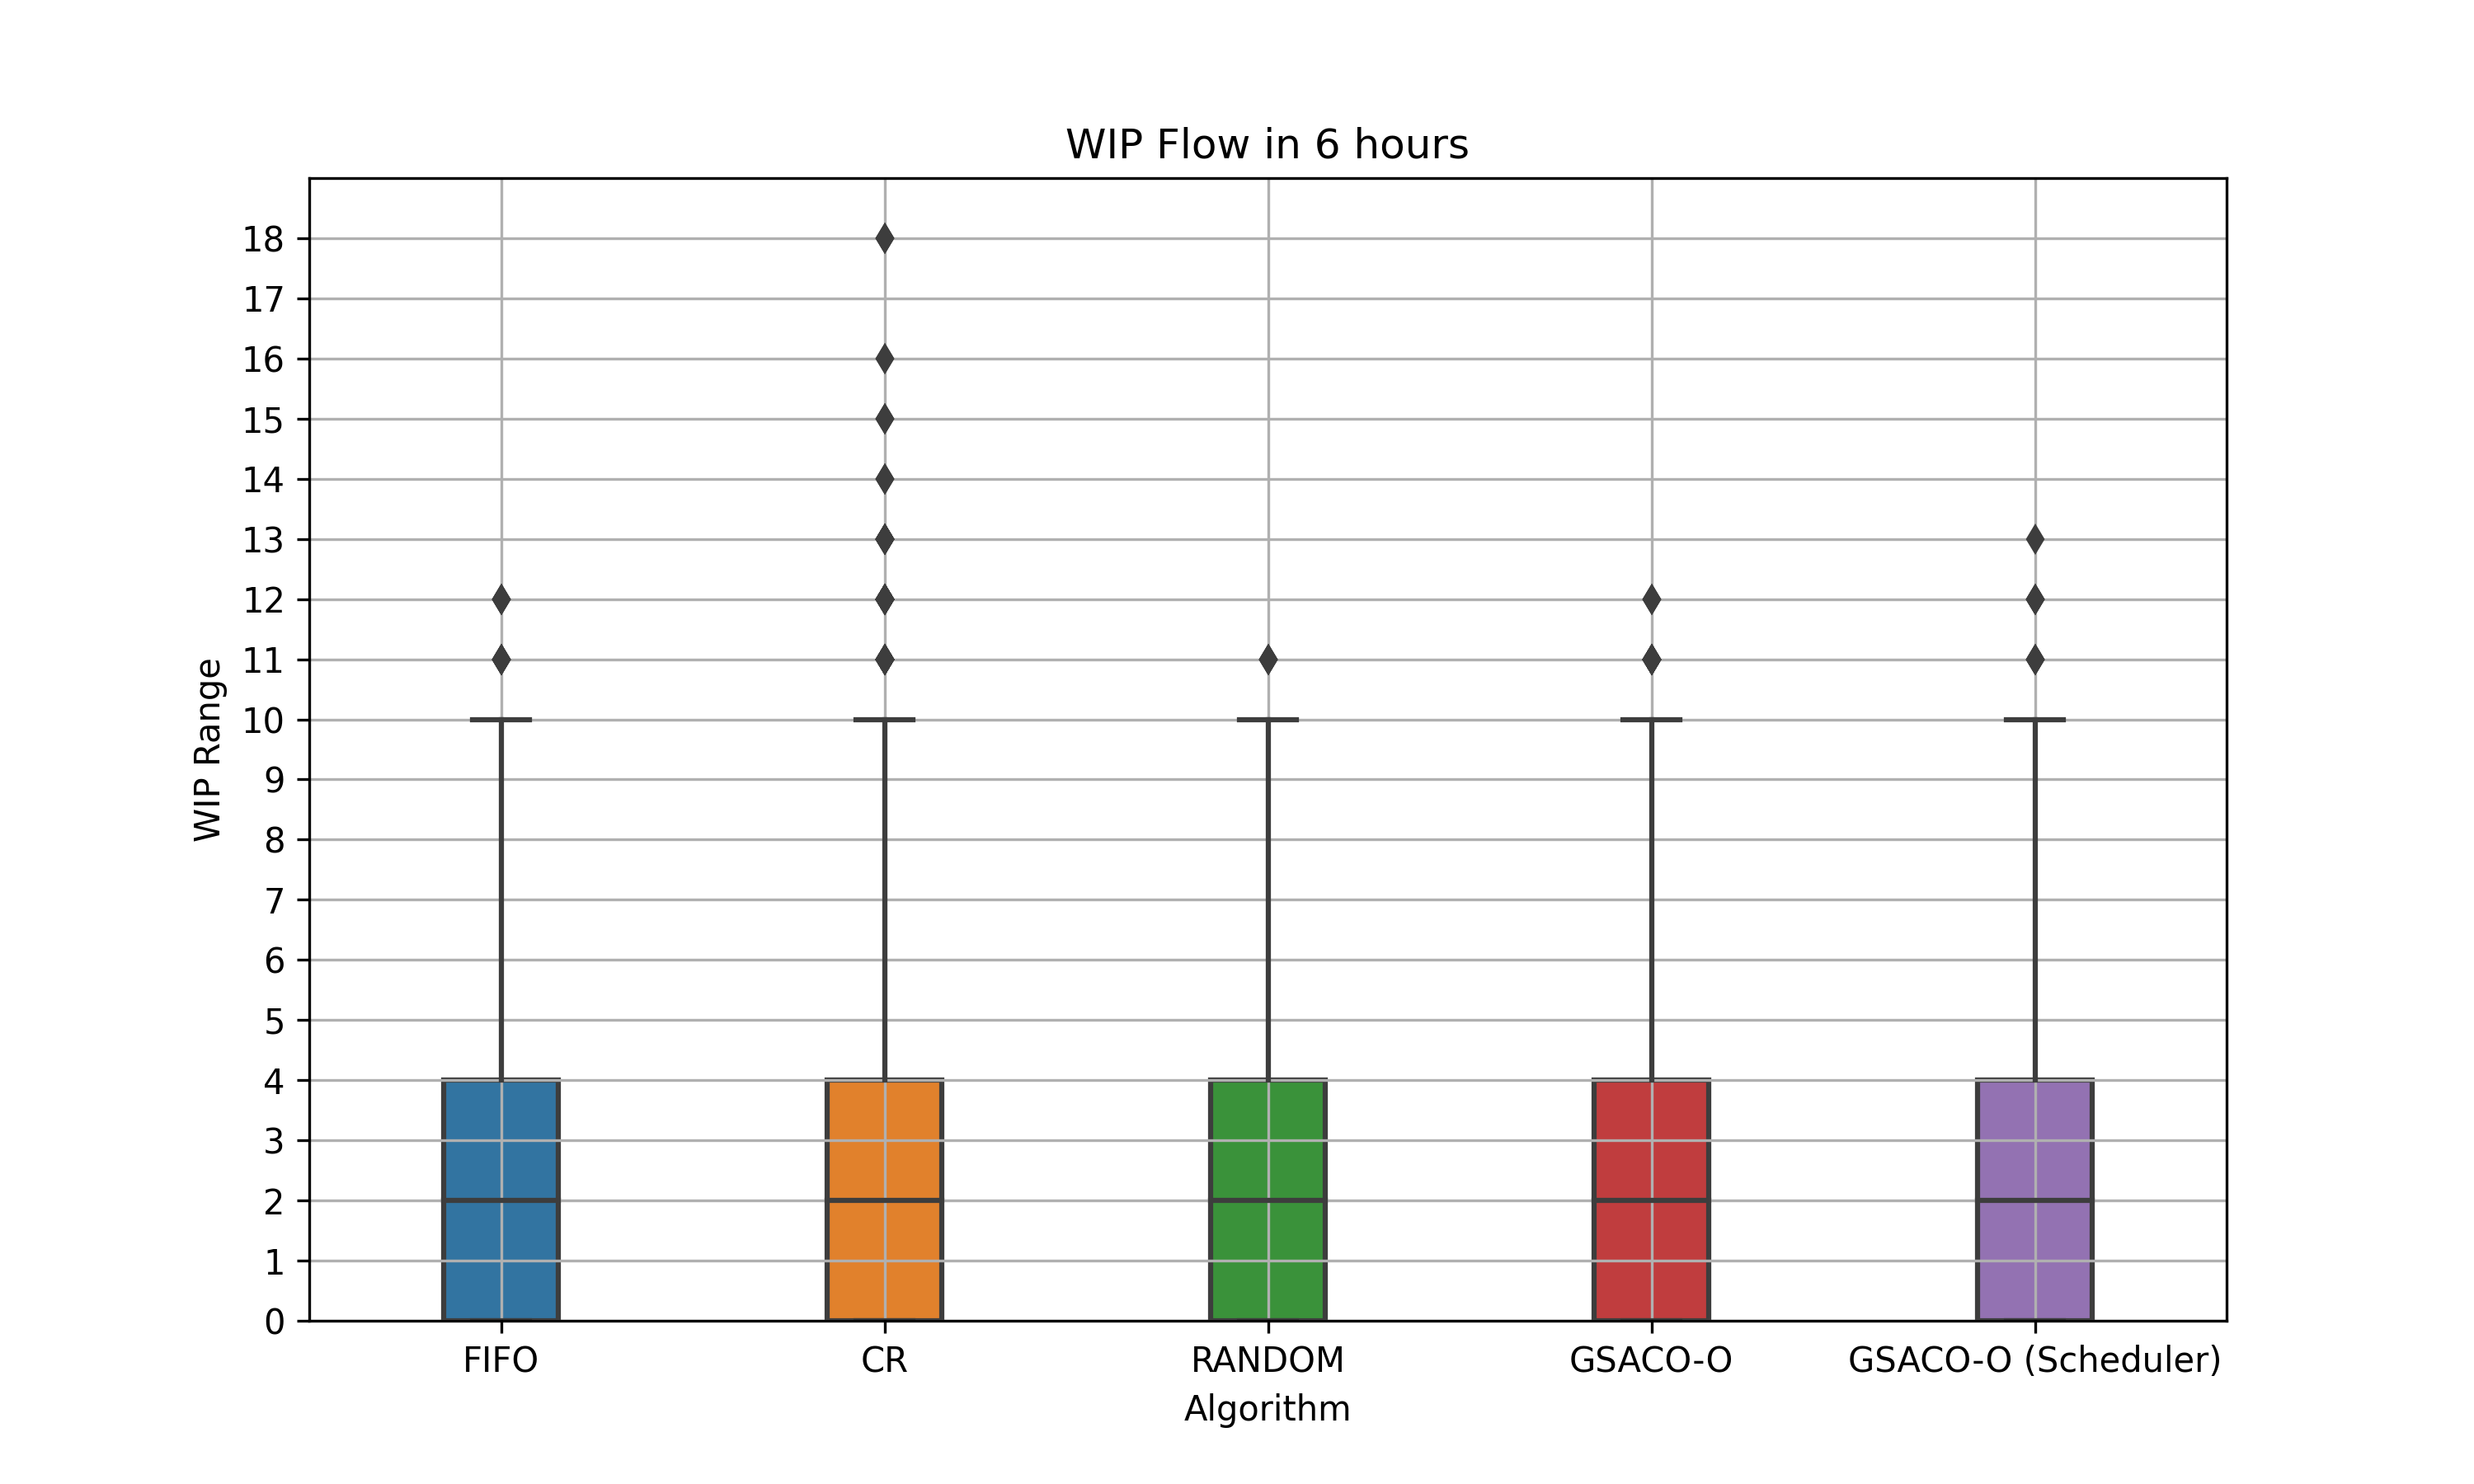
\includegraphics[width=\textwidth]{LVHM/new_period_21600s.png}
		% \caption{}
		% \label{fig:pp6}
	\end{subfigure}
    \caption{WIP flow for LV/HM}
    \label{fig:wip-flows-LVHM}
\end{figure}

The plots in Figure~\ref{fig:wip-flows-LVHM} illustrate the Work in Progress (WIP) flow for LV/HM scenario across various dispatching rules FIFO, CR, RANDOM, GSACO-O and GSACO-O as scheduler over different planning horizons ranging from 1 to 6 hours. Each bar demonstrates the minimum and maximum WIP levels reached during the simulation period under each dispatching rule, with the height of the bar indicating the variability or stability of the WIP flow. 
Across all planning horizons, the range of Work in Progress (WIP) counts is quite consistent across different dispatchers, as represented by FIFO, CR, RANDOM, GSACO-O, and GSACO-O (Scheduler). This suggests that no single dispatcher has a significantly larger WIP range, indicating a balanced approach to managing WIP levels over time.
In case of dispatcher specific observation, FIFO shows the lowest range of WIP variability, suggesting consistent and predictable processing under this rule within the first hour. CR and Random display slightly higher variability, indicating a less stable WIP flow.
Across the longer planning horizons such as 5 and 6 hours, there are more outliers in WIP counts across all dispatchers, which could indicate sporadic spikes in WIP. This trend shows increase in job complexity as the period extends. 
GSACO-O, in both dispatcher and scheduler forms, demonstrates a consistent WIP distribution that does not deviate significantly across time horizons. This indicate that the GSACO-O method is robust in maintaining predictable WIP flows, regardless of operational duration.


\begin{figure}[t]
	\centering
	\begin{subfigure}[b]{0.32\textwidth}
		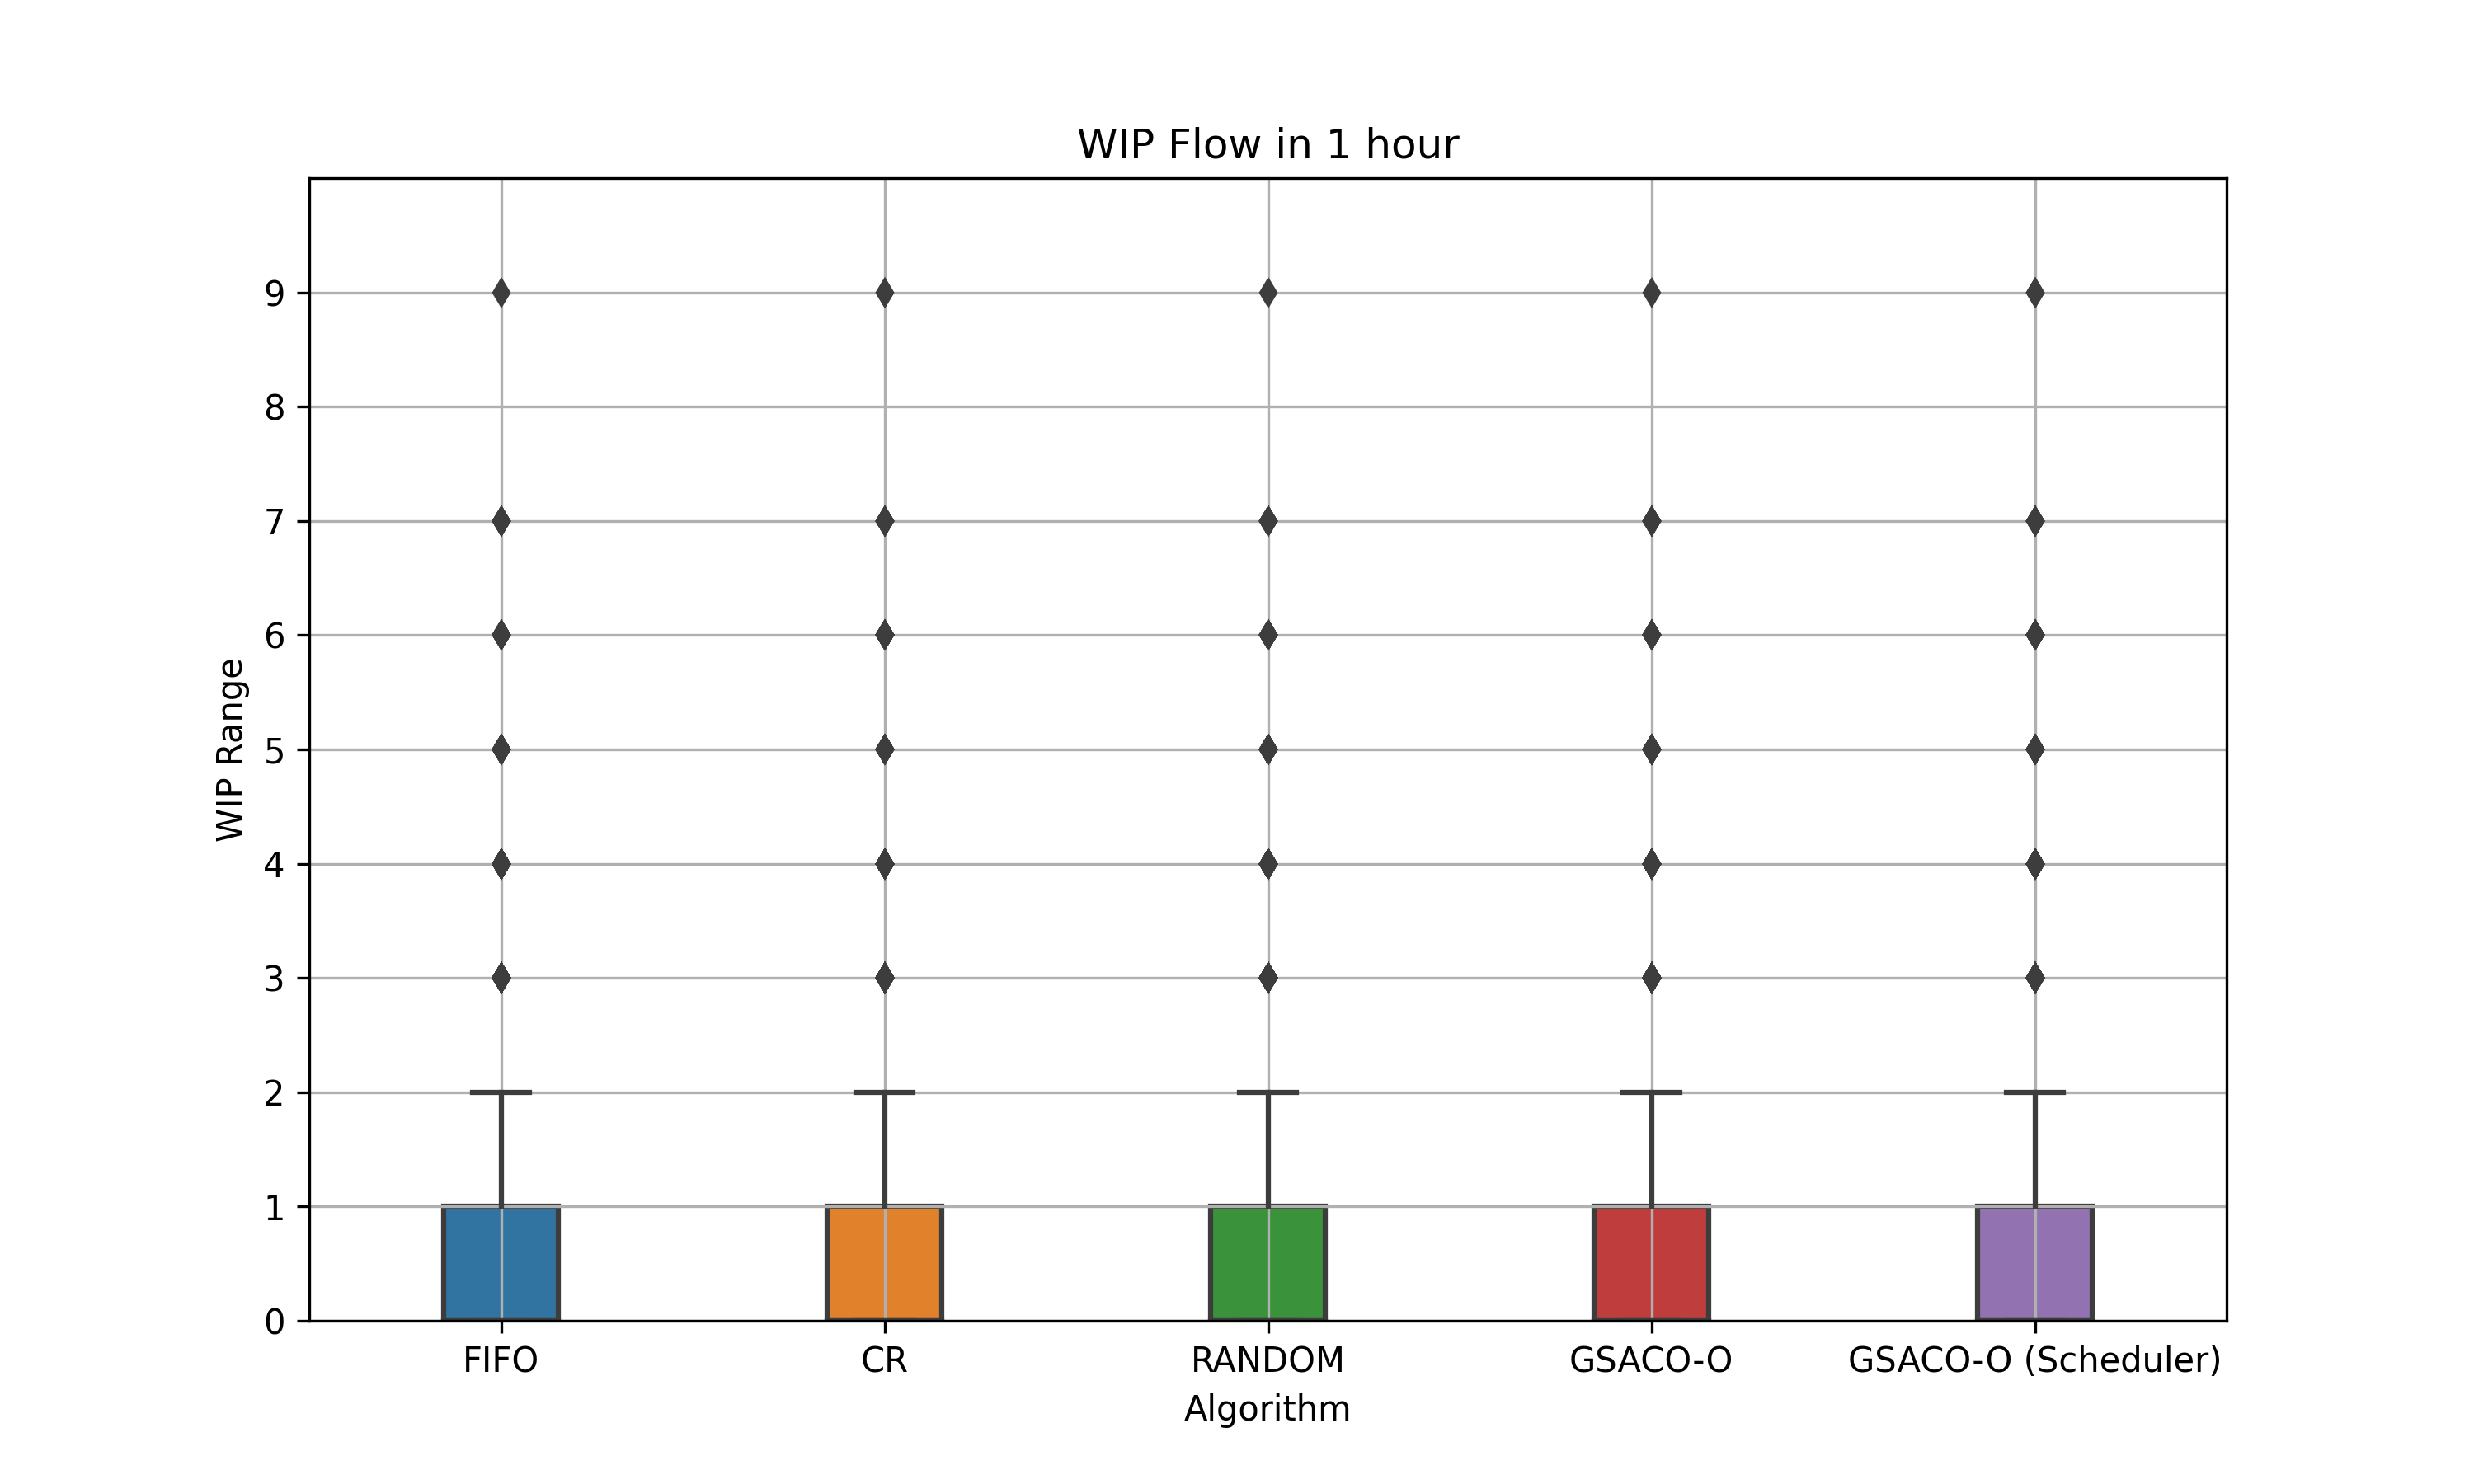
\includegraphics[width=\textwidth]{HVLM/new_period_3600s.png}
		% \caption{}
		% \label{fig:p1}
	\end{subfigure}
	\hfill
	\begin{subfigure}[b]{0.32\textwidth}
		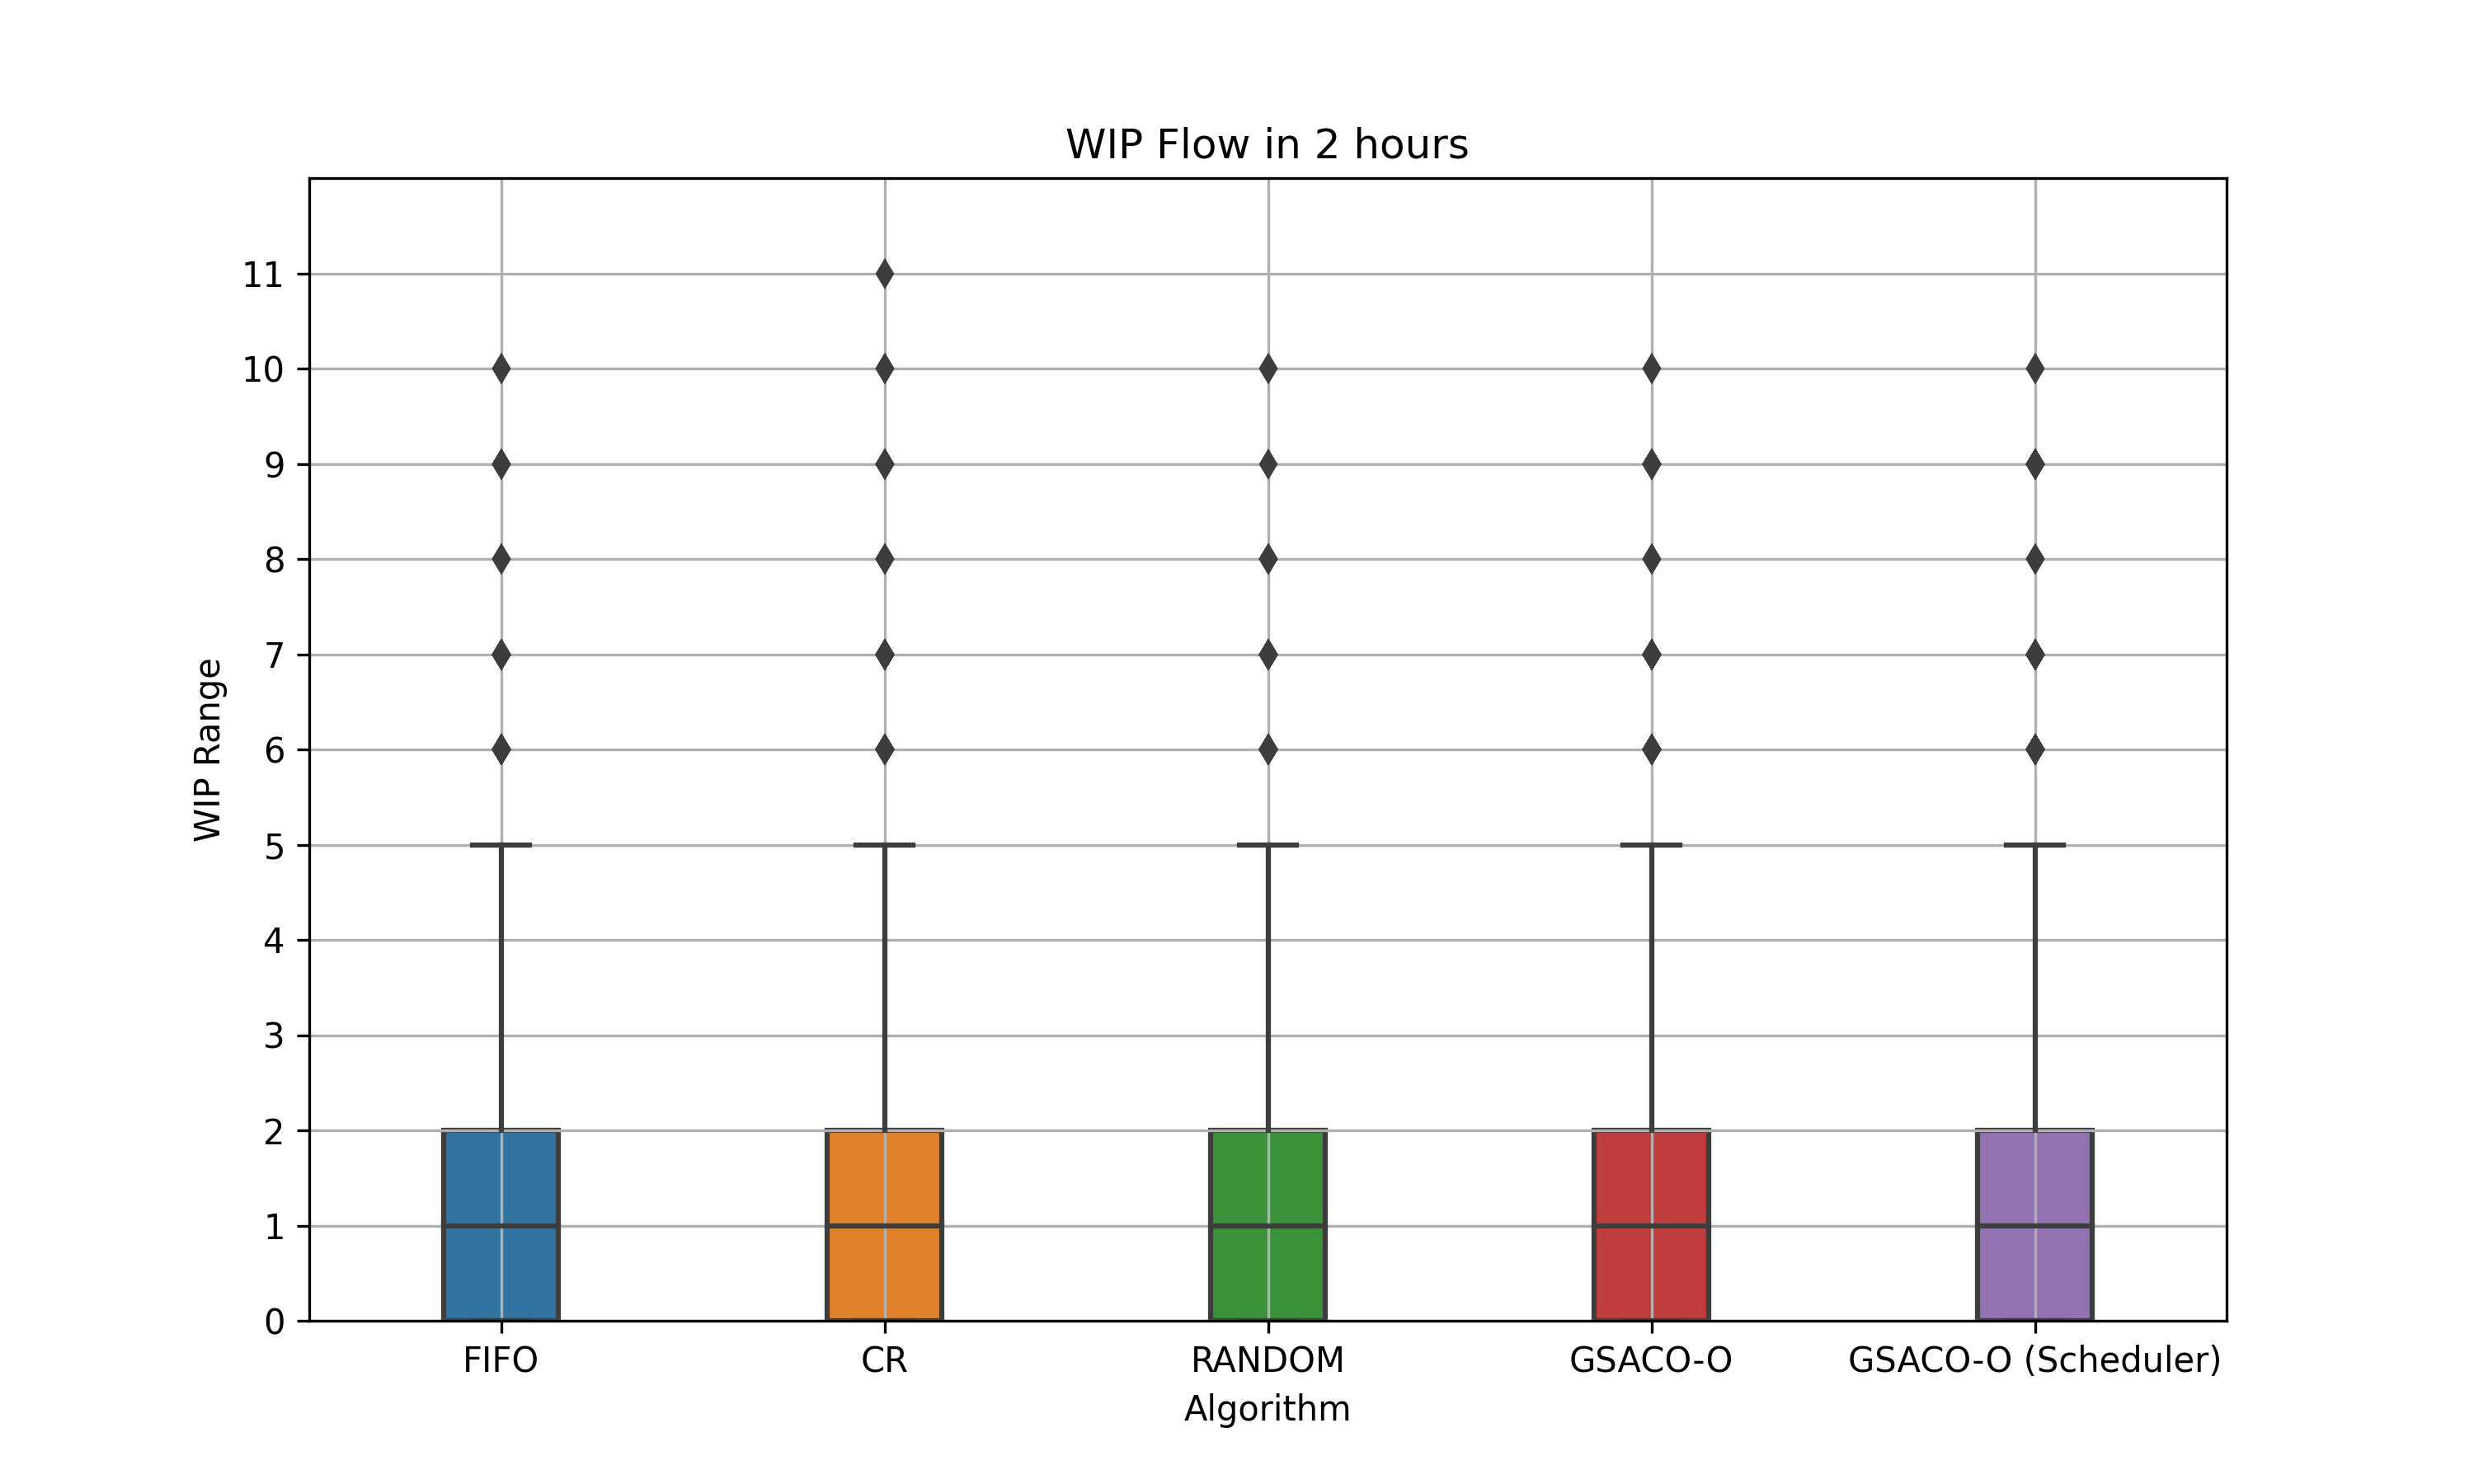
\includegraphics[width=\textwidth]{HVLM/new_period_7200s.png}
		% \caption{}
		% \label{fig:p2}
	\end{subfigure}
	\hfill
	\begin{subfigure}[b]{0.32\textwidth}
		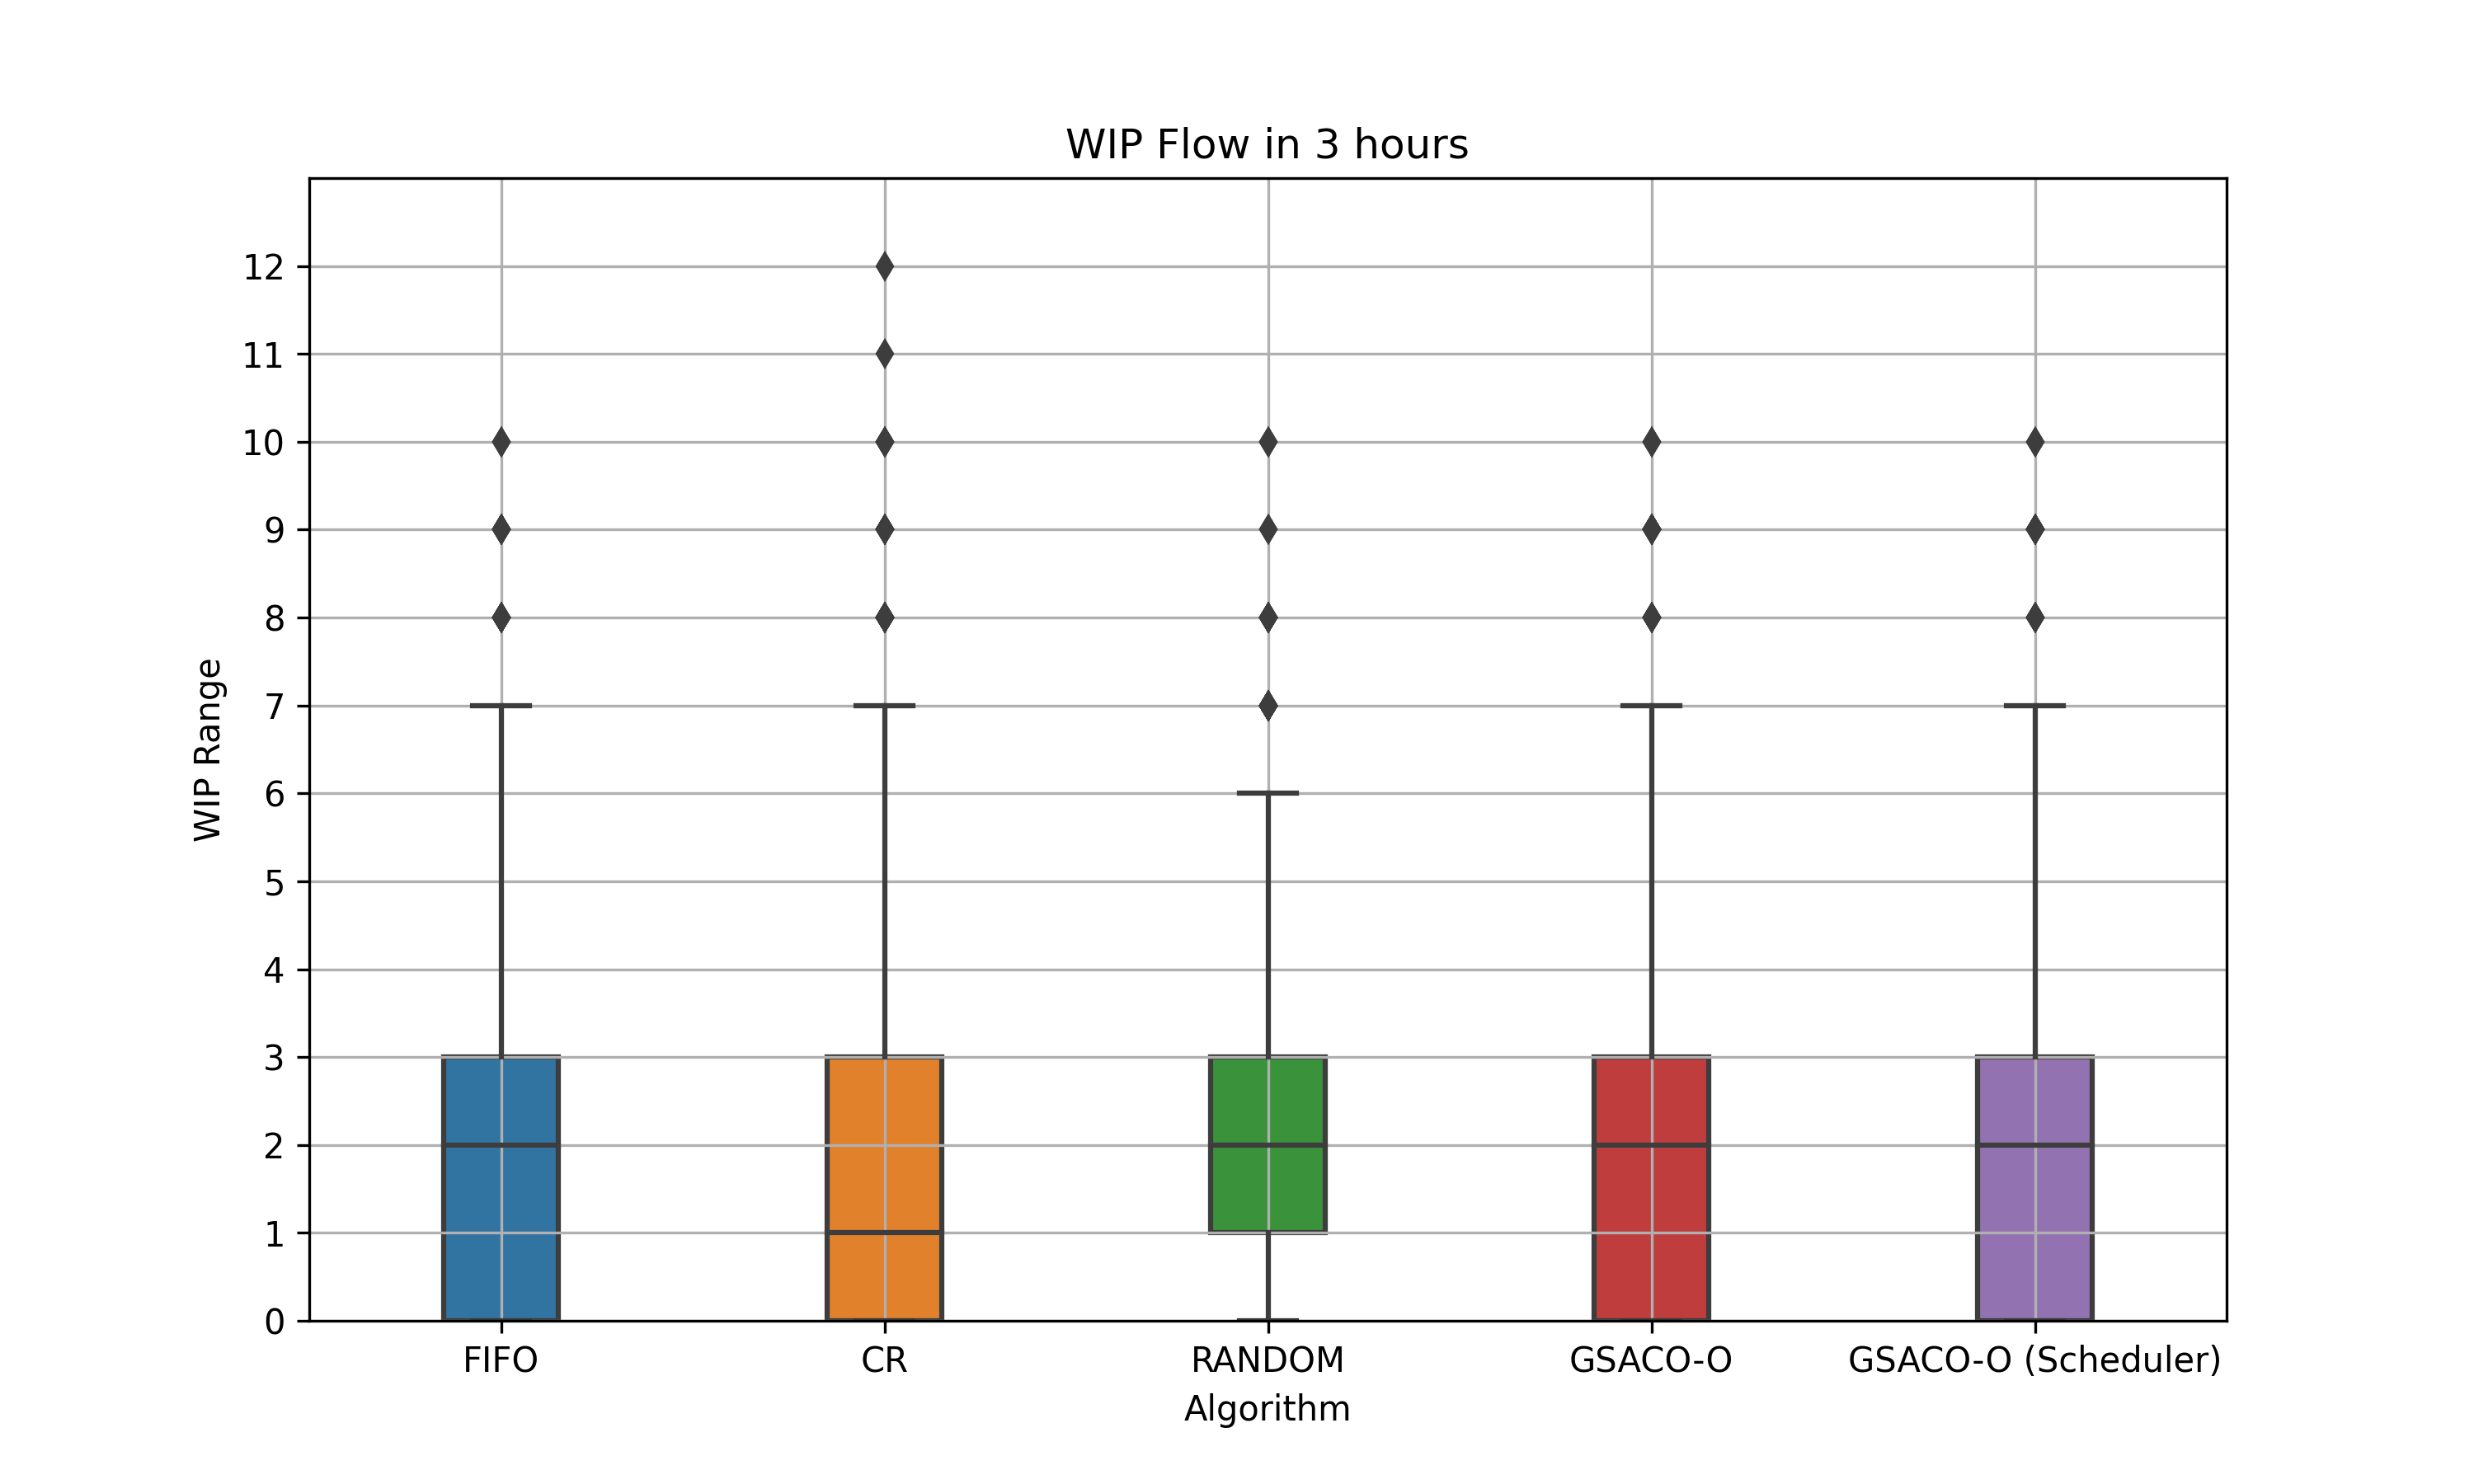
\includegraphics[width=\textwidth]{HVLM/new_period_10800s.png}
		% \caption{}
		% \label{fig:p3}
	\end{subfigure}
	
	\begin{subfigure}[b]{0.32\textwidth}
		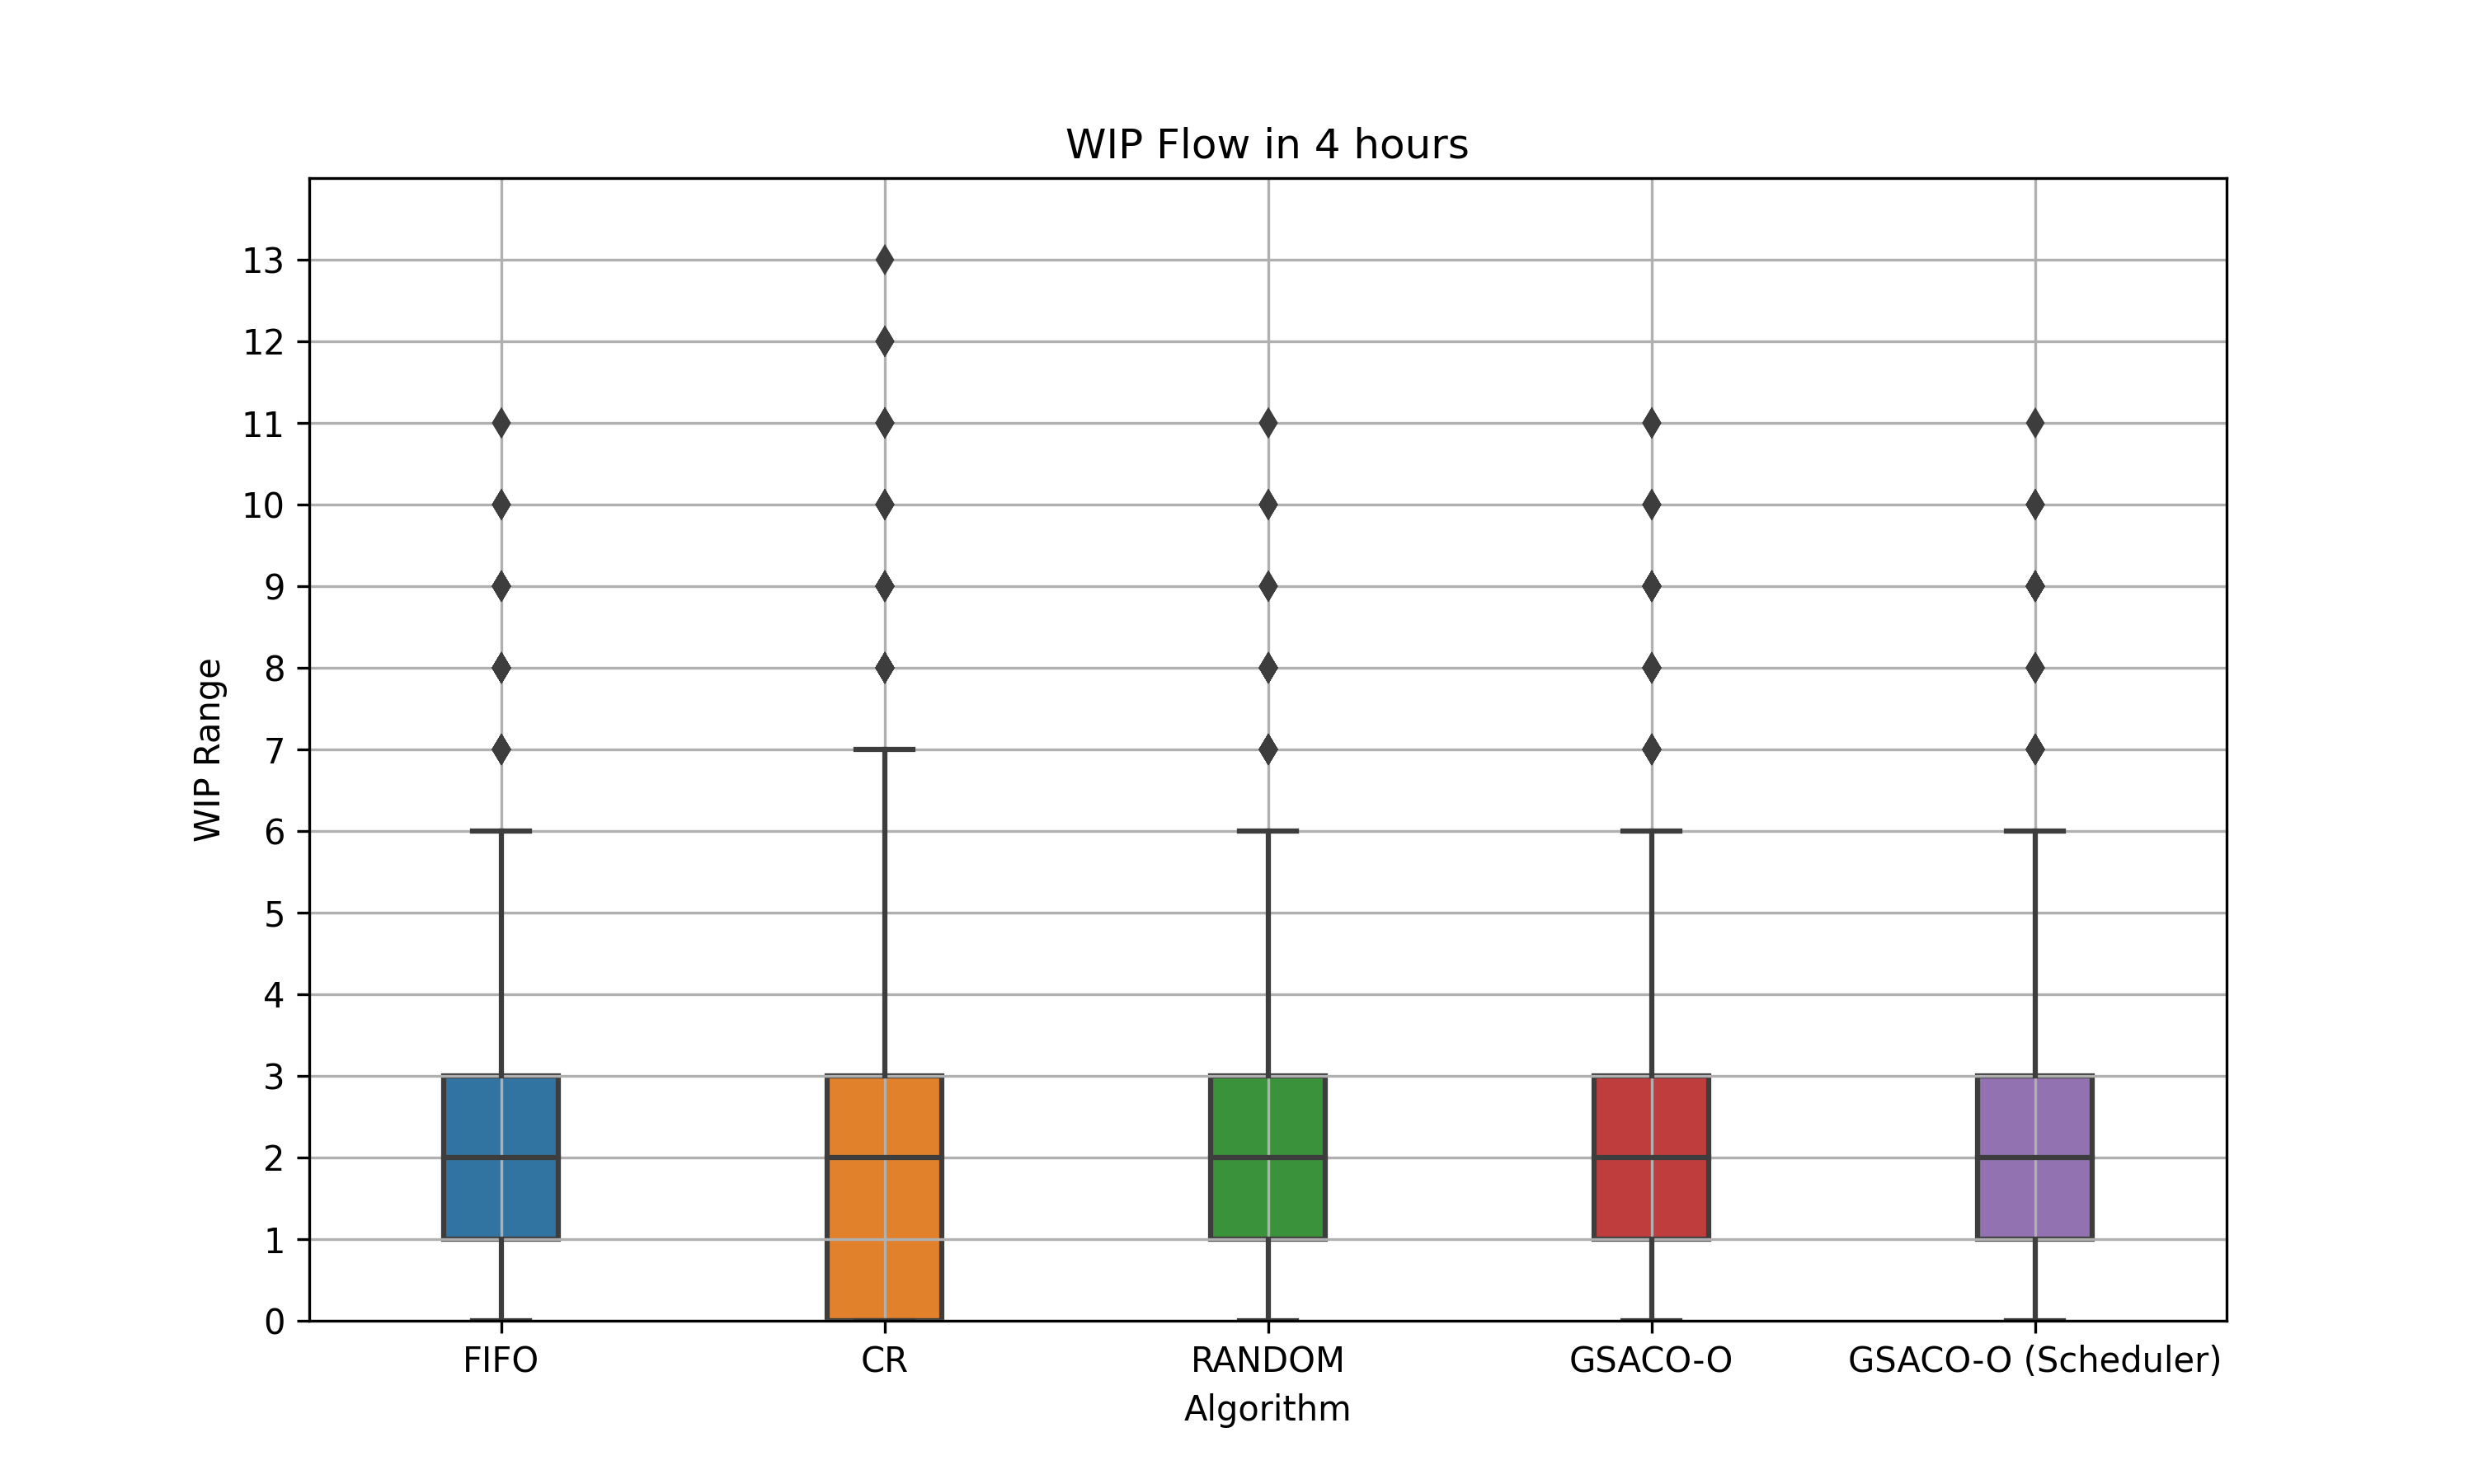
\includegraphics[width=\textwidth]{HVLM/new_period_14400s.png}
		% \caption{}
		% \label{fig:p4}
	\end{subfigure}
	\hfill
	\begin{subfigure}[b]{0.32\textwidth}
		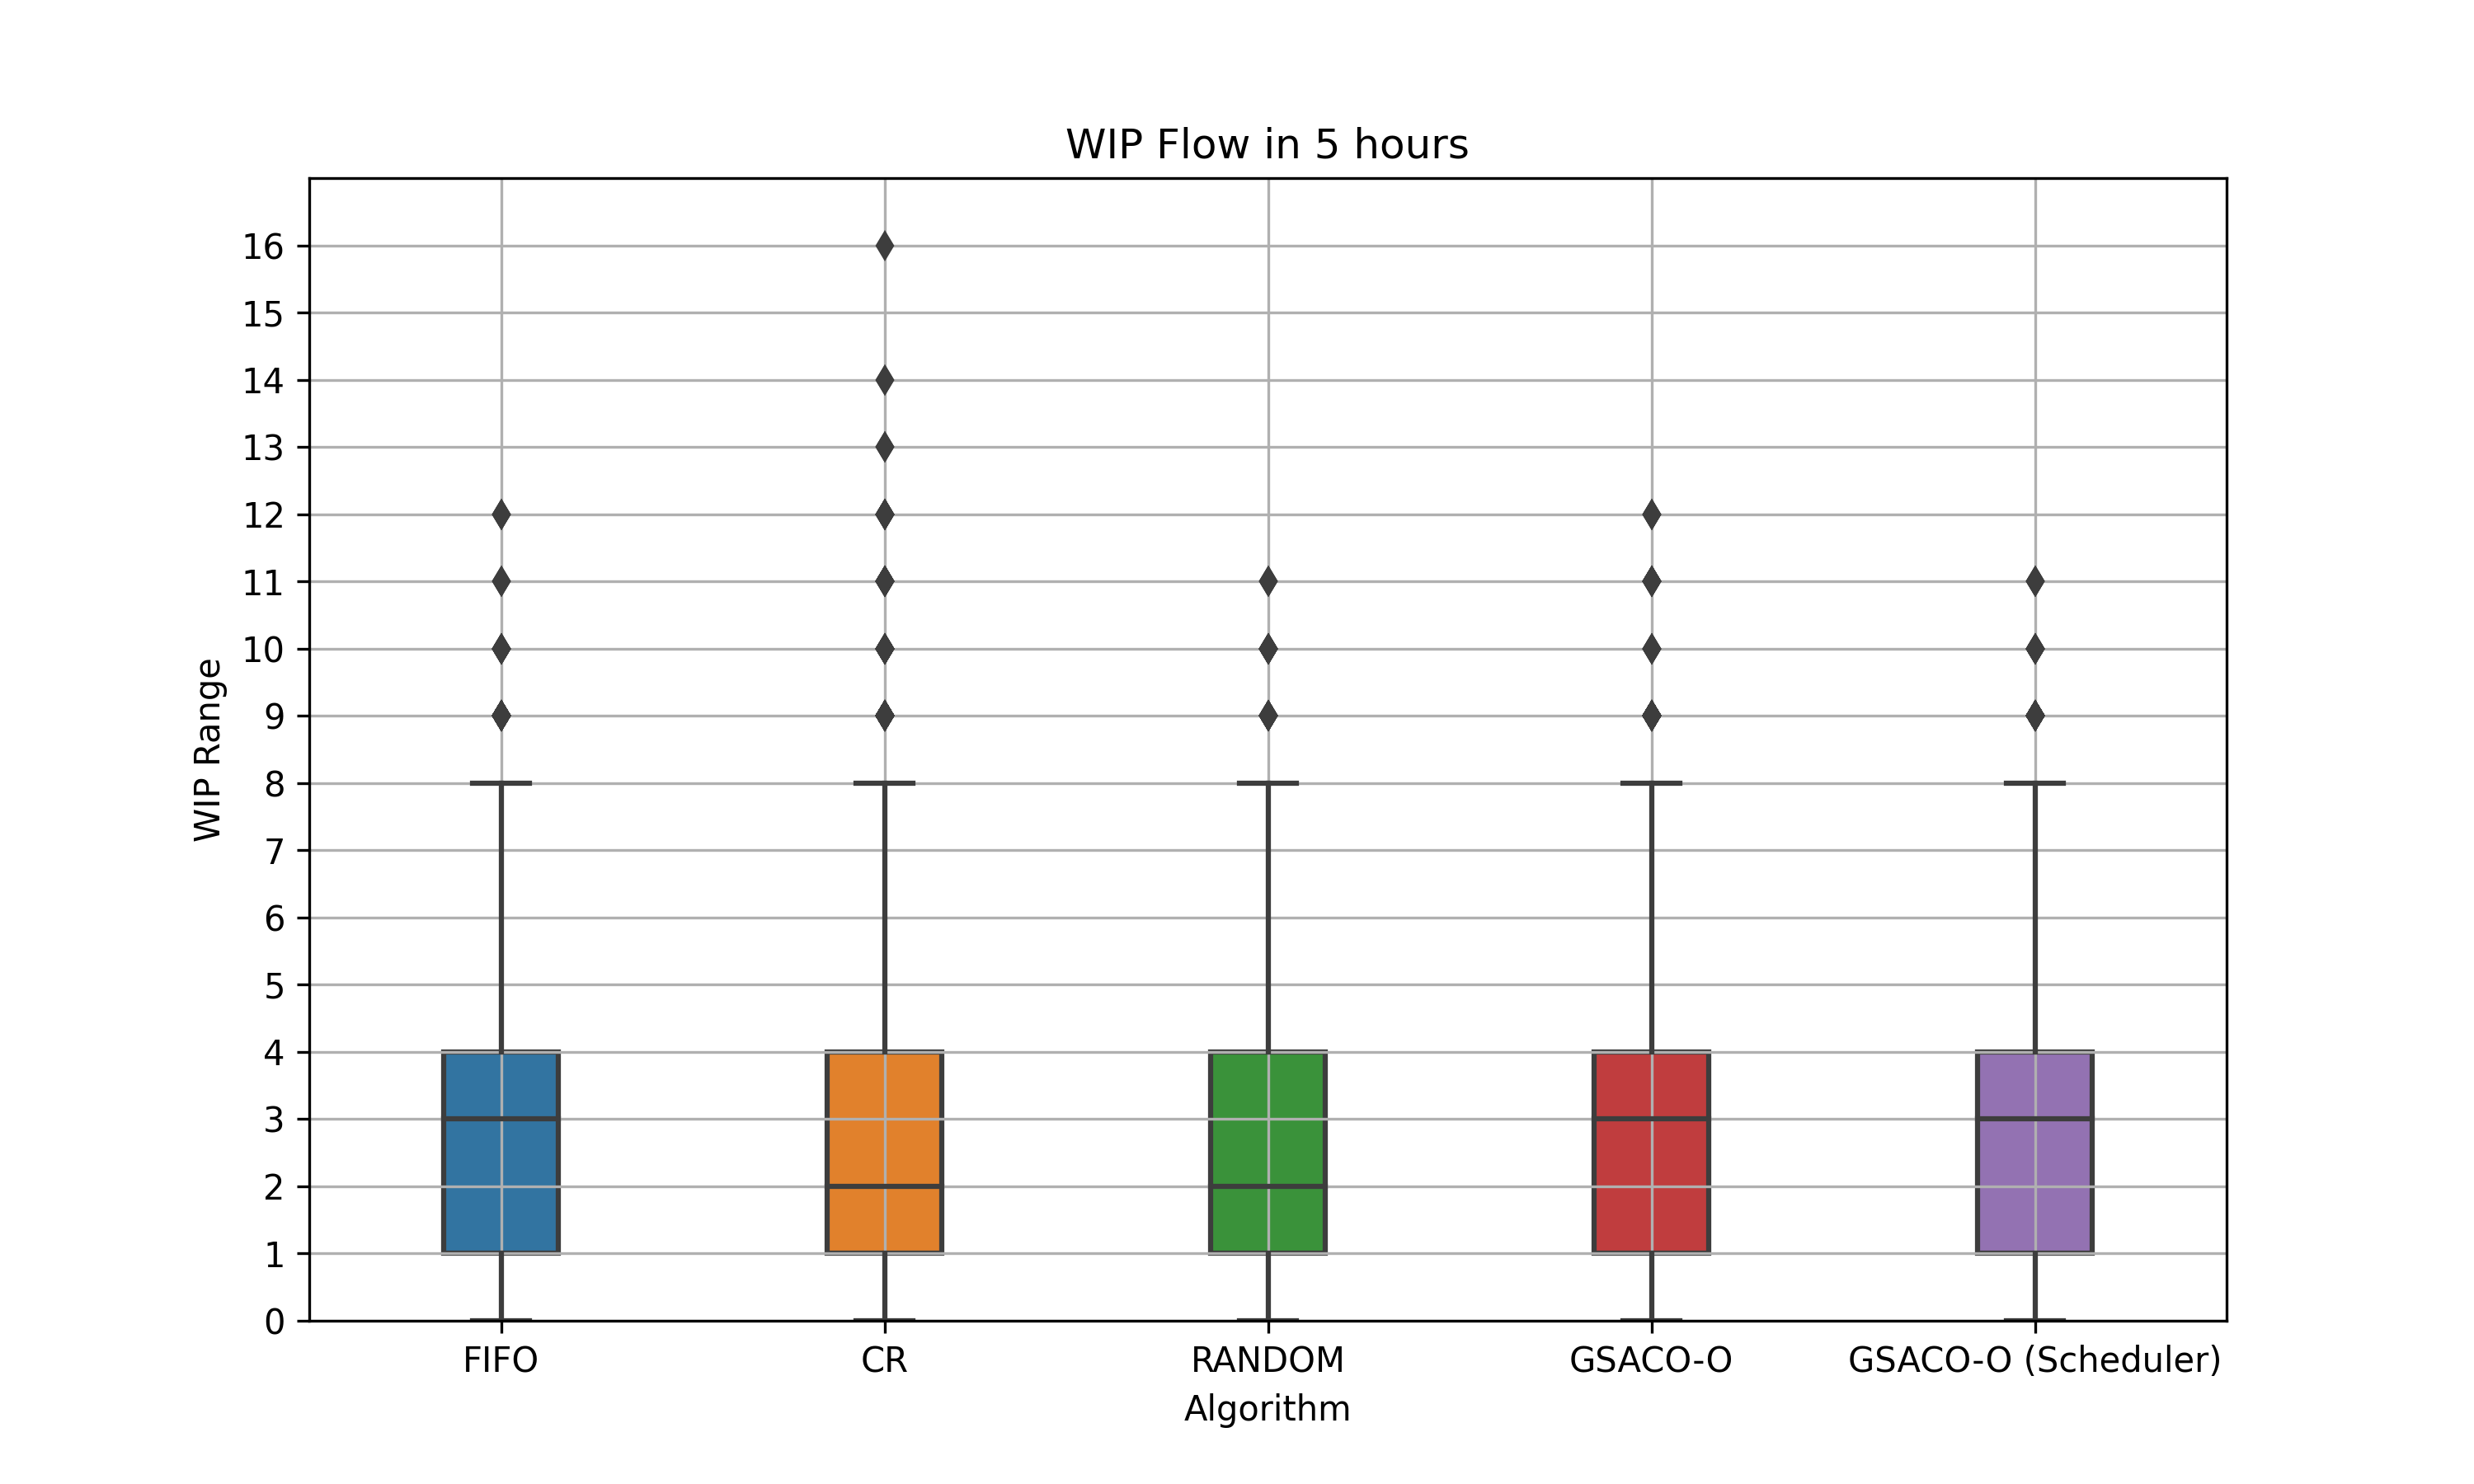
\includegraphics[width=\textwidth]{HVLM/new_period_18000s.png}
		% \caption{}
		% \label{fig:p5}
	\end{subfigure}
	\hfill
	\begin{subfigure}[b]{0.32\textwidth}
		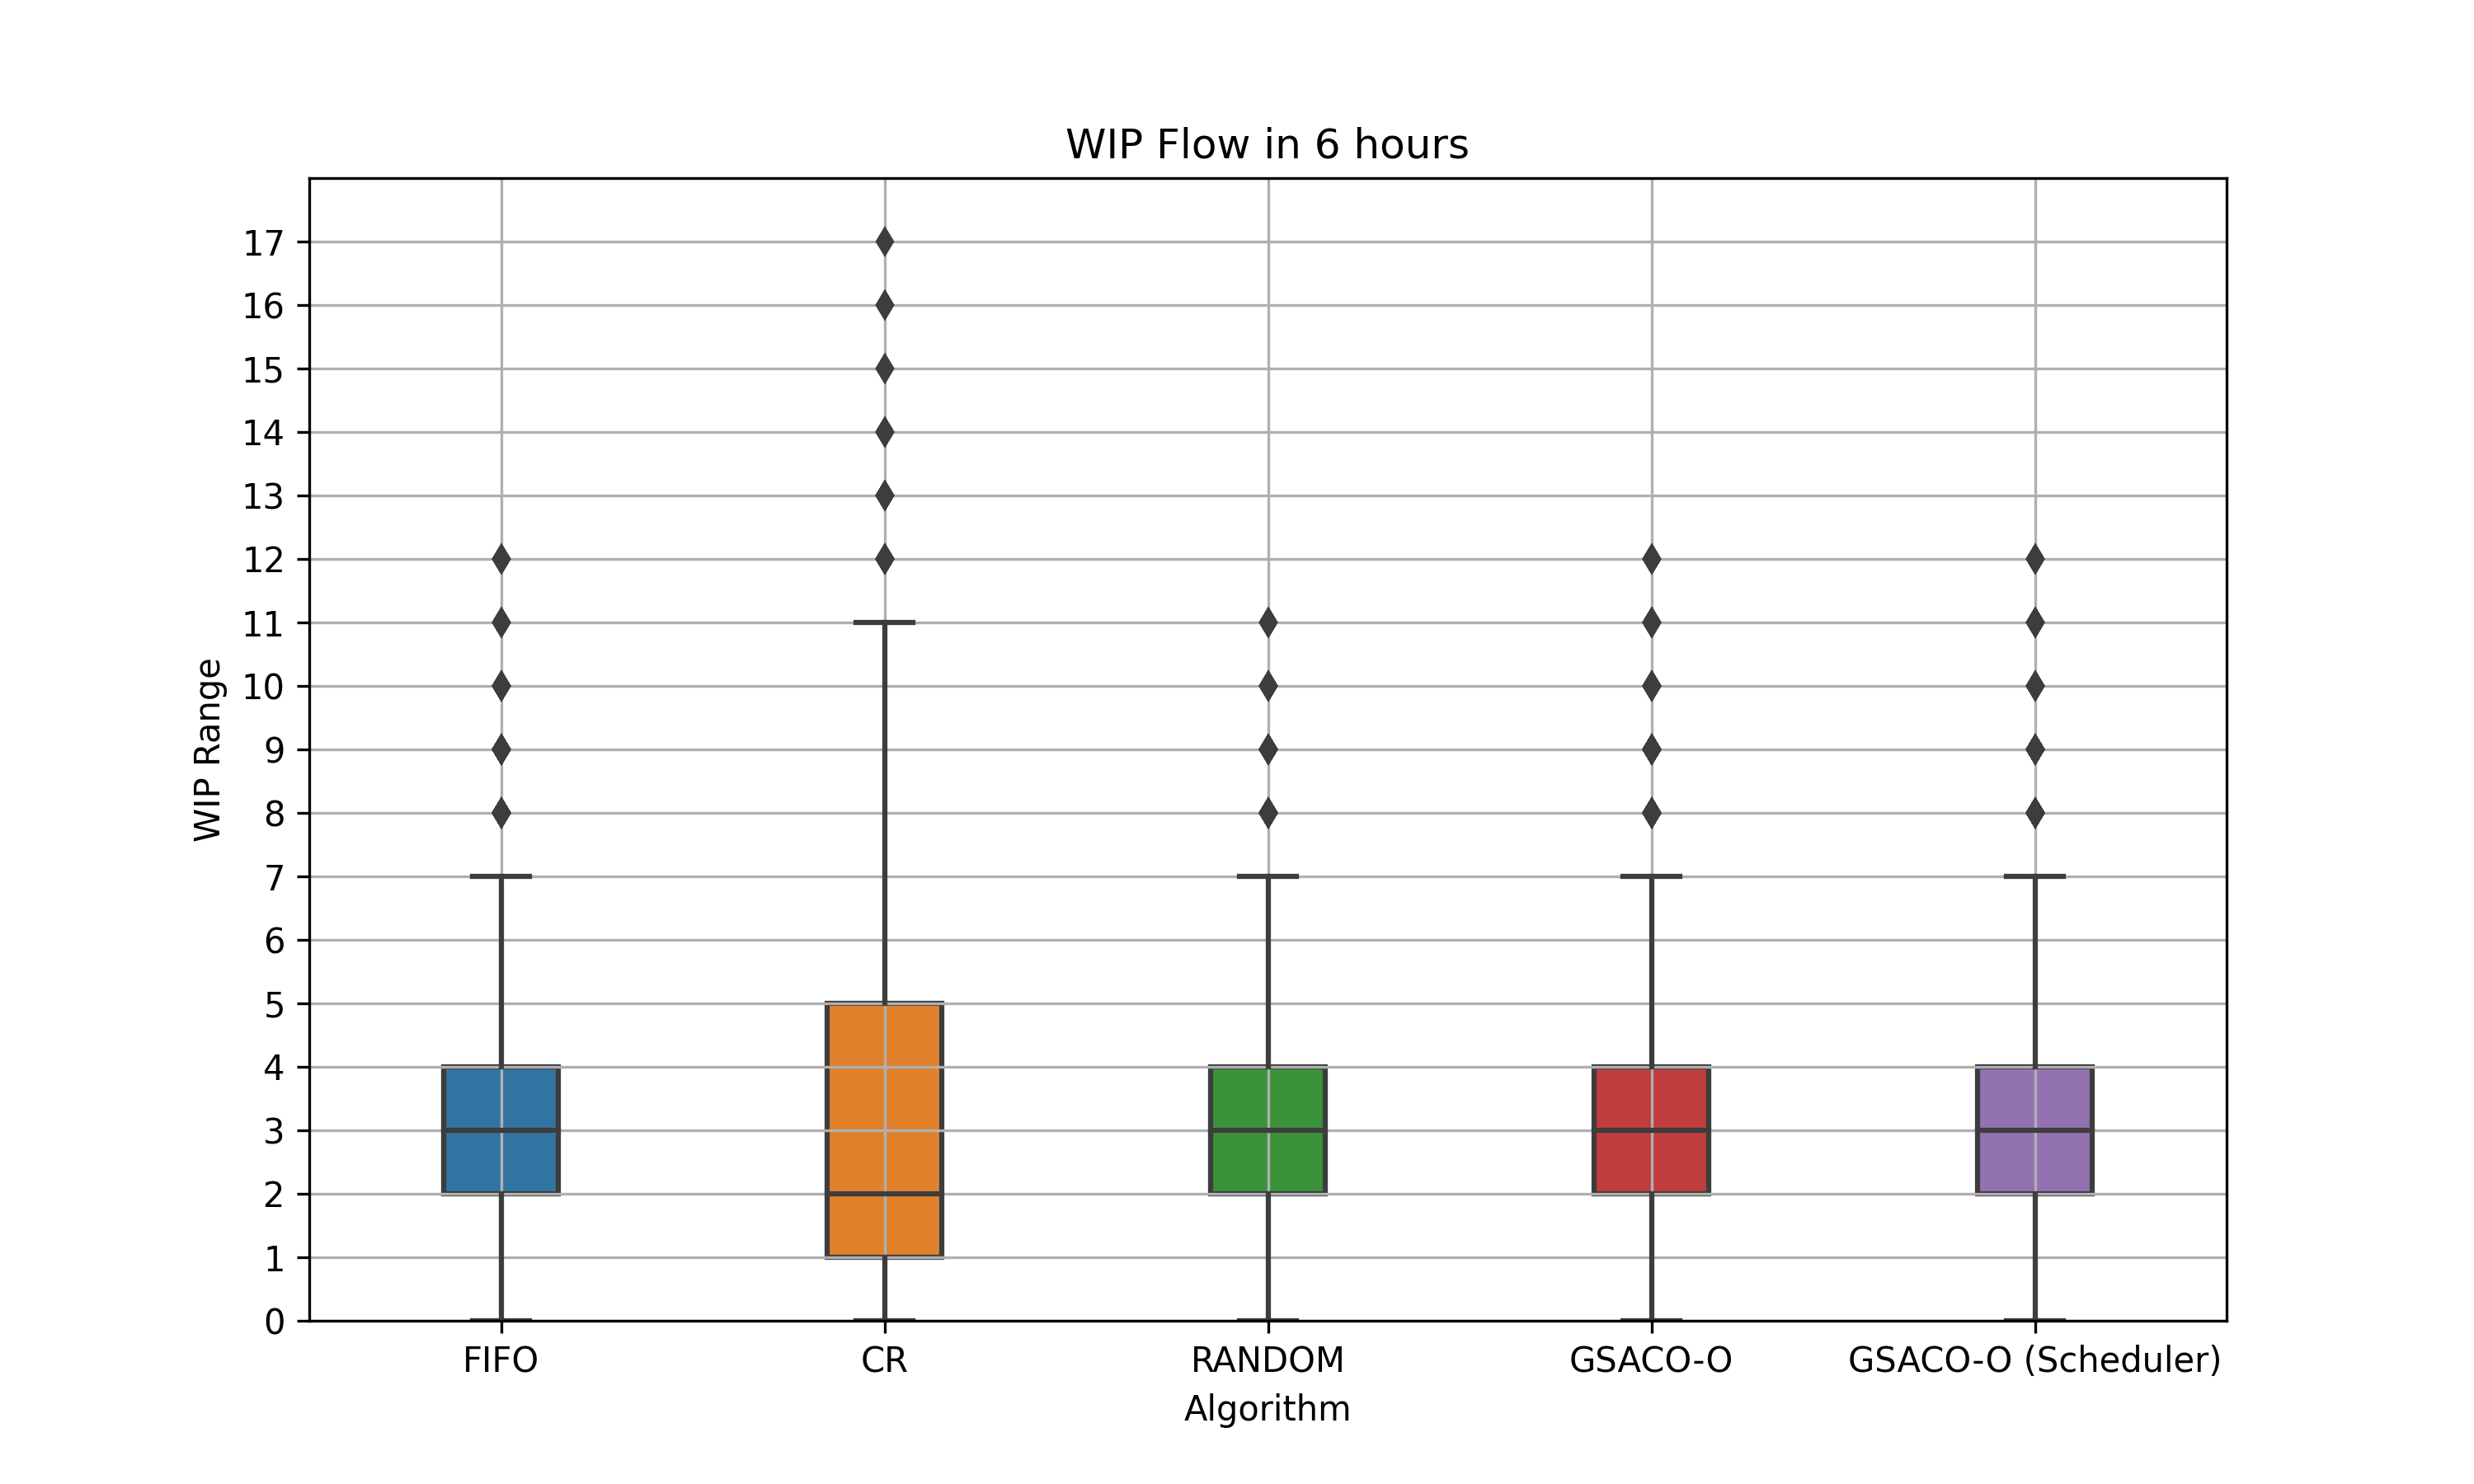
\includegraphics[width=\textwidth]{HVLM/new_period_21600s.png}
		% \caption{}
		% \label{fig:p6}
	\end{subfigure}
	\caption{WIP flow for HV/LM}
	\label{fig:wip-flows-HVLM}
\end{figure}

Similarly, the plots in Figure~\ref{fig:wip-flows-HVLM} illustrate the Work in Progress (WIP) flow for HV/LM scenario. The FIFO dispatcher maintains a narrow interquartile range (IQR) and a relatively low WIP count in comparison to other dispatchers.
Even at 6 hours, FIFO’s WIP values are less dispersed than other algorithms, indicating a conservative and stable approach in managing WIP.
The CR dispatcher shows a slightly wider IQR than FIFO, especially noticeable in the 5th and 6th hour plots.
The RANDOM dispatcher has a consistent distribution similar to FIFO. Its WIP values increase consistently across longer planning hours, suggesting a flexible approach that does not tightly control WIP levels and makes it less predictable.
GSACO-O, when used as a dispatcher, shows a stable and controlled WIP range similar to FIFO and CR but with some incremental flexibility.
Across the time periods, GSACO-O maintains a low median and narrow IQR, suggesting an efficient handling of WIP without significant spikes. GSACO-O as a scheduler demonstrates similar behavior to its dispatcher, with low variability in WIP values.

In conclusion, the comparative analysis across different dispatching algorithms (FIFO, CR, RANDOM, GSACO-O as dispatcher, and GSACO-O as scheduler) reveals distinct characteristics in WIP handling as planning horizons extend from 1 to 6 hours.
GSACO-O, whether used as a dispatcher or scheduler, consistently demonstrates robust performance with stable WIP ranges and limited outliers, suggesting a reliable choice for applications requiring predictability in WIP levels. FIFO and CR also show controlled WIP distributions but with slightly more variability in extended periods, indicating that while they maintain order, they might face occasional increases in WIP as time progresses. RANDOM, by contrast, allows more variability, with a slightly wider IQR and an increasing number of outliers in longer horizons, which reflects a more flexible but less controlled approach to WIP management.
As planning horizons extend, all algorithms experience a rise in WIP counts and outliers, highlighting the impact of prolonged operational periods on workload variability. For scenarios prioritizing stability and predictability, GSACO-O and FIFO emerge as preferred choices.

Additionally, if WIP levels remain consistent across dispatching strategies, using a scheduler like GSACO-O could be computationally expensive without significant benefit in WIP performance. In such cases, opting for a dispatcher approach rather than a scheduler could reduce computational overhead while achieving similar WIP outcomes. These insights can guide the selection of dispatching and scheduling algorithms in settings where managing WIP levels is crucial to operational efficiency and workflow stability, with computational cost considerations also taken into account.
















